\PassOptionsToPackage{prologue,dvipsnames}{xcolor}
\documentclass{article} % For LaTeX2e
\usepackage{iclr2025_conference,times}

% Optional math commands from https://github.com/goodfeli/dlbook_notation.
\input{math_commands.tex}

\usepackage[dvipsnames]{xcolor}
%\usepackage{cancel}
\usepackage{hyperref}
\hypersetup{colorlinks,
           linkcolor=NavyBlue,
           urlcolor=NavyBlue,
           citecolor=NavyBlue}

\usepackage{url}
\usepackage{graphicx}
\usepackage{tabu}
\usepackage{booktabs}
\usepackage{multirow}
\usepackage{colortbl}
\usepackage{subcaption}
\usepackage[font=small]{caption}
\usepackage{wrapfig}
\usepackage{arydshln} 
\usepackage{makecell}
\usepackage{stfloats}
\usepackage{array}
\usepackage[hang,flushmargin]{footmisc}
\usepackage{wasysym}
\usepackage{listings}
\usepackage{cleveref}
%
% --- inline annotations
%
\usepackage[dvipsnames]{xcolor}
\newcommand{\red}[1]{{\color{red}#1}}
\newcommand{\todo}[1]{{\color{red}#1}}
\newcommand{\TODO}[1]{\textbf{\color{red}[TODO: #1]}}
\newcommand{\weidi}[1]{{\textcolor{magenta}{weidi: #1} }}
\newcommand{\DSZ}[1]{{\textcolor{blue}{#1}}}
% \newcommand{\DSZ}[1]{{#1}}
% --- disable by uncommenting  
% \renewcommand{\TODO}[1]{}
% \renewcommand{\todo}[1]{#1}

\definecolor{mygreen}{RGB}{29, 177, 0}
\definecolor{darkgreen}{rgb}{0.0, 0.5, 0.0}

\def\ourmethod{ReKV}

\newcommand{\plusvalue}[1]{\hspace{0.2em}\textcolor{darkgreen}{\textbf{\scriptsize{(+#1)}}}}
\newcommand{\minusvalue}[1]{\hspace{0.2em}\textcolor{red}{\textbf{\scriptsize{(-#1)}}}}
\newcommand{\retrieve}[2]{#1 FPS $\to$ #2 Frames}

\title{Streaming Video Question-Answering with \\In-context Video KV-Cache Retrieval}

% Authors must not appear in the submitted version. They should be hidden
% as long as the \iclrfinalcopy macro remains commented out below.
% Non-anonymous submissions will be rejected without review.

\author{
Shangzhe Di$^{1,2}$
\quad
Zhelun Yu$^{2}$
\quad
Guanghao Zhang$^{2}$
\quad
Haoyuan Li$^{2}$
\quad
Tao Zhong$^{2}$
\\
\textbf{
Hao Cheng$^{2}$
\quad
Bolin Li$^{2}$
\quad
Wanggui He$^{2}$
\quad
Fangxun Shu$^{2}$
\quad
Hao Jiang$^{2}$
}
\vspace{3pt}
\\
$^{1}$Shanghai Jiao Tong University \quad $^{2}$Alibaba Group
\\
\texttt{dishangzhe@sjtu.edu.cn}
}

% The \author macro works with any number of authors. There are two commands
% used to separate the names and addresses of multiple authors: \And and \AND.
%
% Using \And between authors leaves it to \LaTeX{} to determine where to break
% the lines. Using \AND forces a linebreak at that point. So, if \LaTeX{}
% puts 3 of 4 authors names on the first line, and the last on the second
% line, try using \AND instead of \And before the third author name.

\newcommand{\fix}{\marginpar{FIX}}
\newcommand{\new}{\marginpar{NEW}}

\iclrfinalcopy % Uncomment for camera-ready version, but NOT for submission.
\begin{document}

\maketitle

\begin{abstract}
\noindent Recent advancements in Multimodal Large Language Models (MLLMs) have demonstrated significant improvement in offline video understanding. However, extending these capabilities to streaming video inputs, remains challenging, as existing models struggle to simultaneously maintain stable understanding performance, real-time responses, and low GPU memory overhead. To address this challenge, we propose \hermes, a novel training-free architecture for real-time and accurate understanding of video streams. Based on a mechanistic attention investigation, we conceptualize KV cache as a hierarchical memory framework that encapsulates video information across multiple granularities. During inference, \hermes reuses a compact KV cache, enabling efficient streaming understanding under resource constraints. Notably, \hermes requires no auxiliary computations upon the arrival of user queries, thereby guaranteeing real-time responses for continuous video stream interactions, which achieves 10$\times$ faster TTFT compared to prior SOTA. Even when reducing video tokens by up to 68\% compared with uniform sampling, \hermes achieves superior or comparable accuracy across all benchmarks, with up to 11.4\% gains on streaming datasets.
\end{abstract}
% 为了方便修改,我们可以先定义一个统一的高度变量
\newlength{\myfigheight}
\setlength{\myfigheight}{7.01cm} % 在这里统一调整三张图的高度

\begin{figure*}[t]
    \centering
    
    % --- 子图 (a) ---
    \begin{subfigure}{\widthof{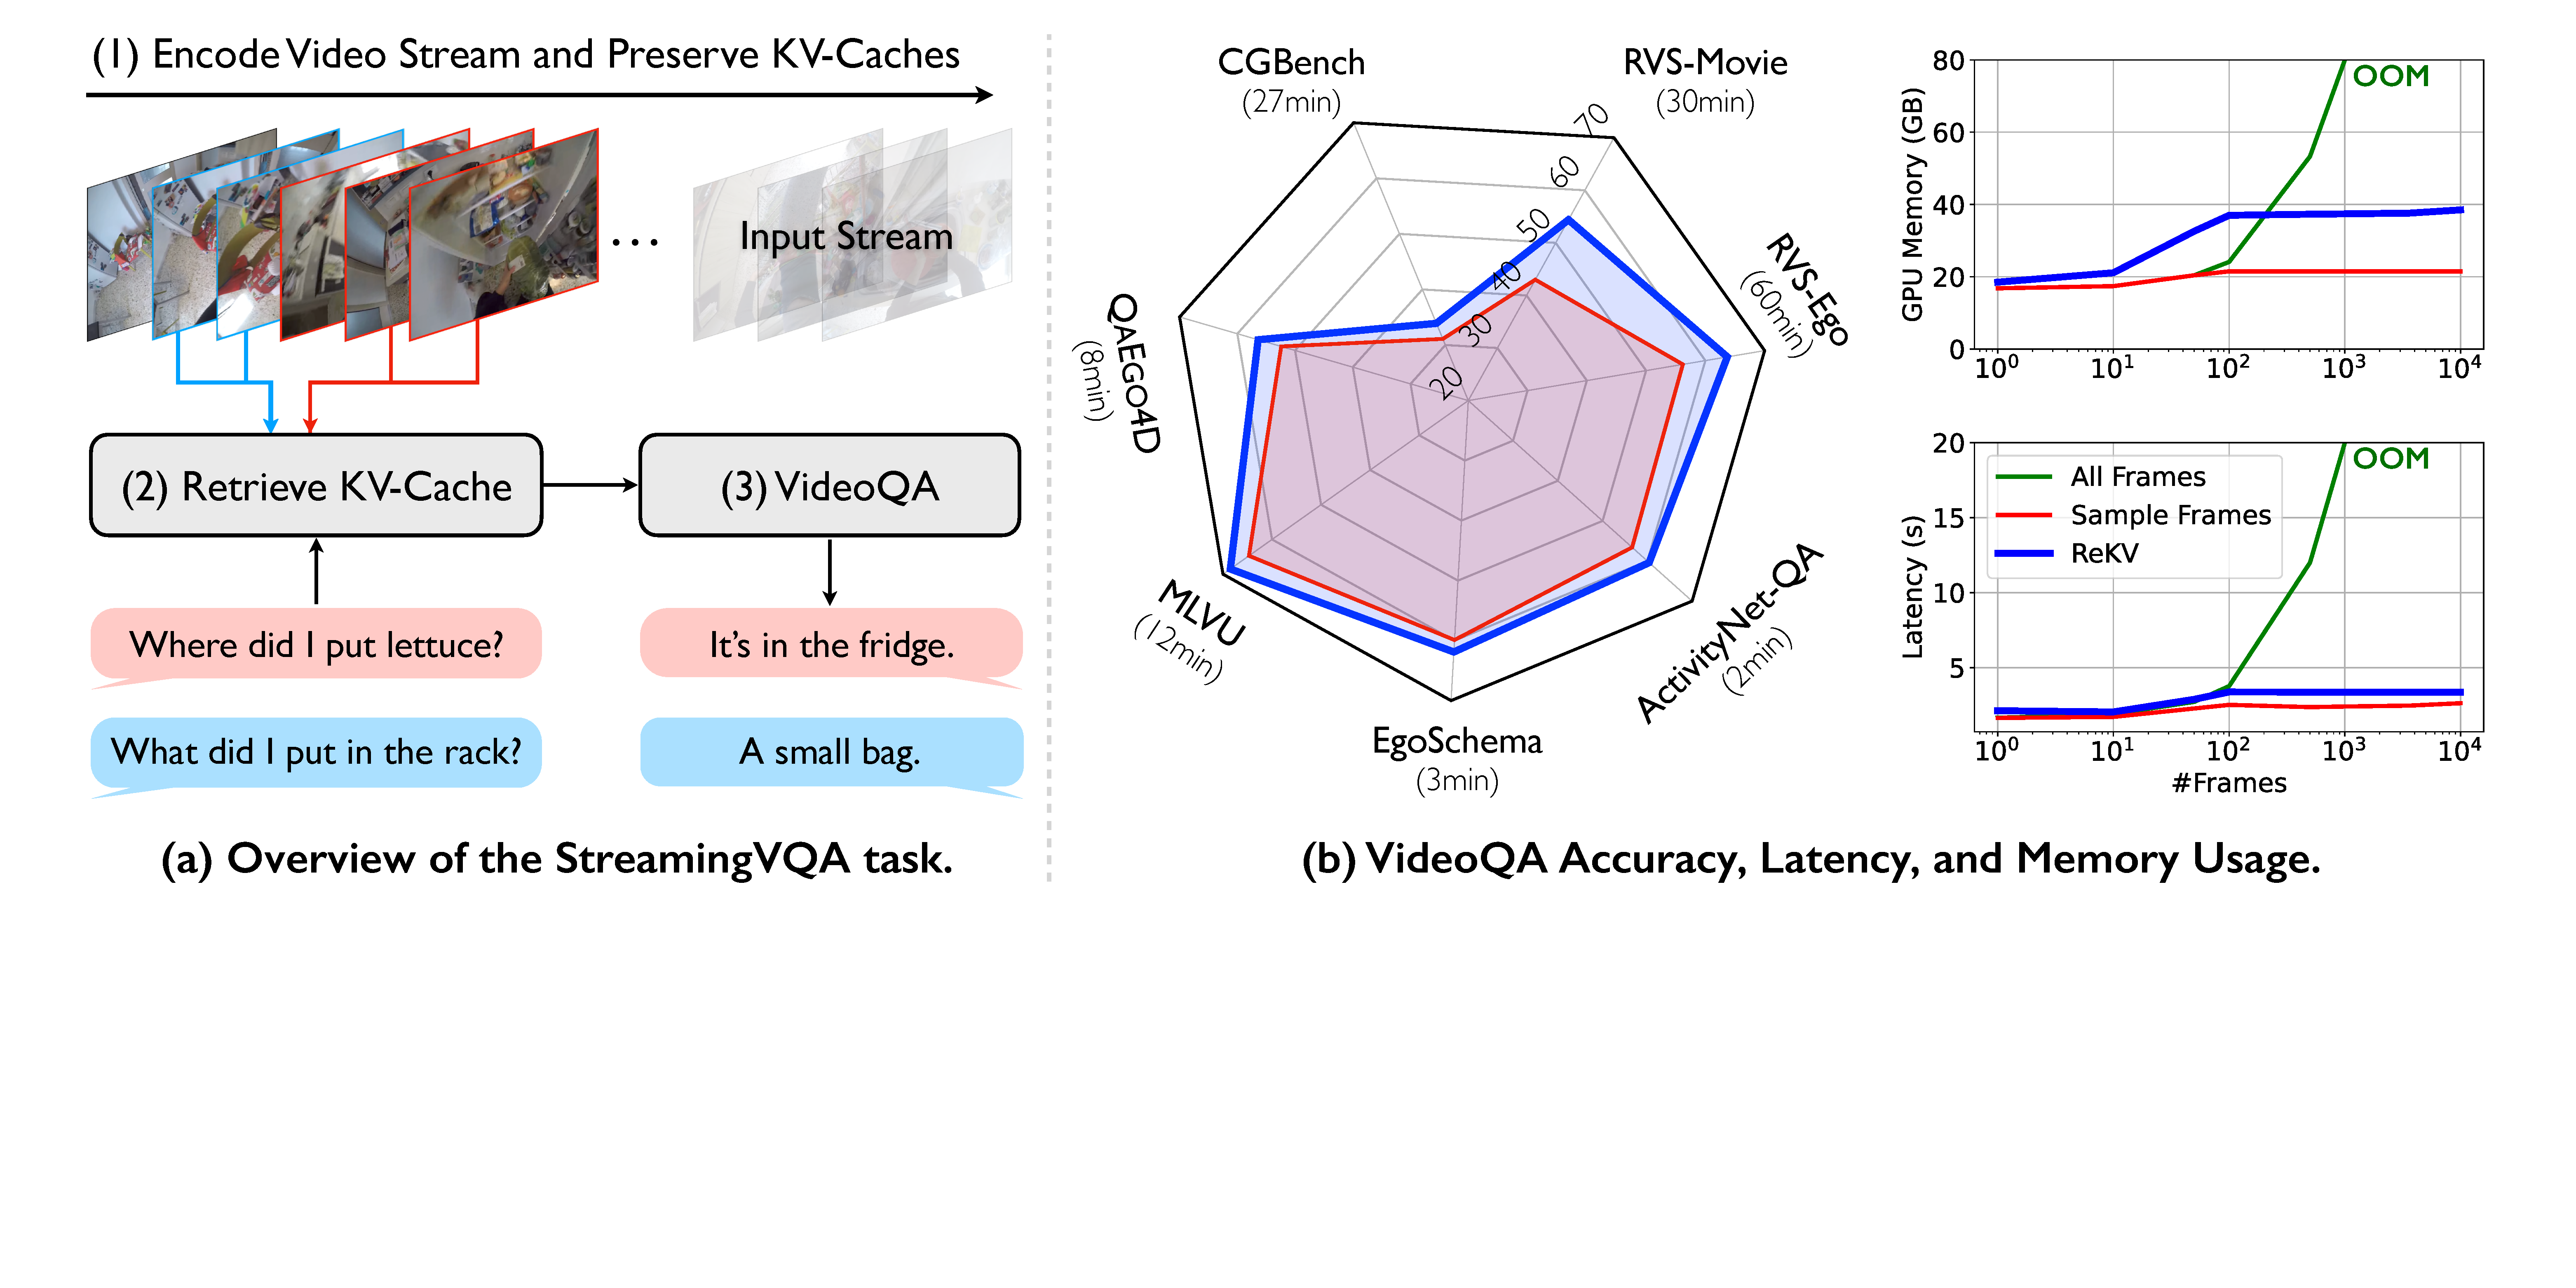
\includegraphics[height=\myfigheight, trim={0 0 415pt 0}, clip]{figures/teaser.pdf}}}
        \centering
        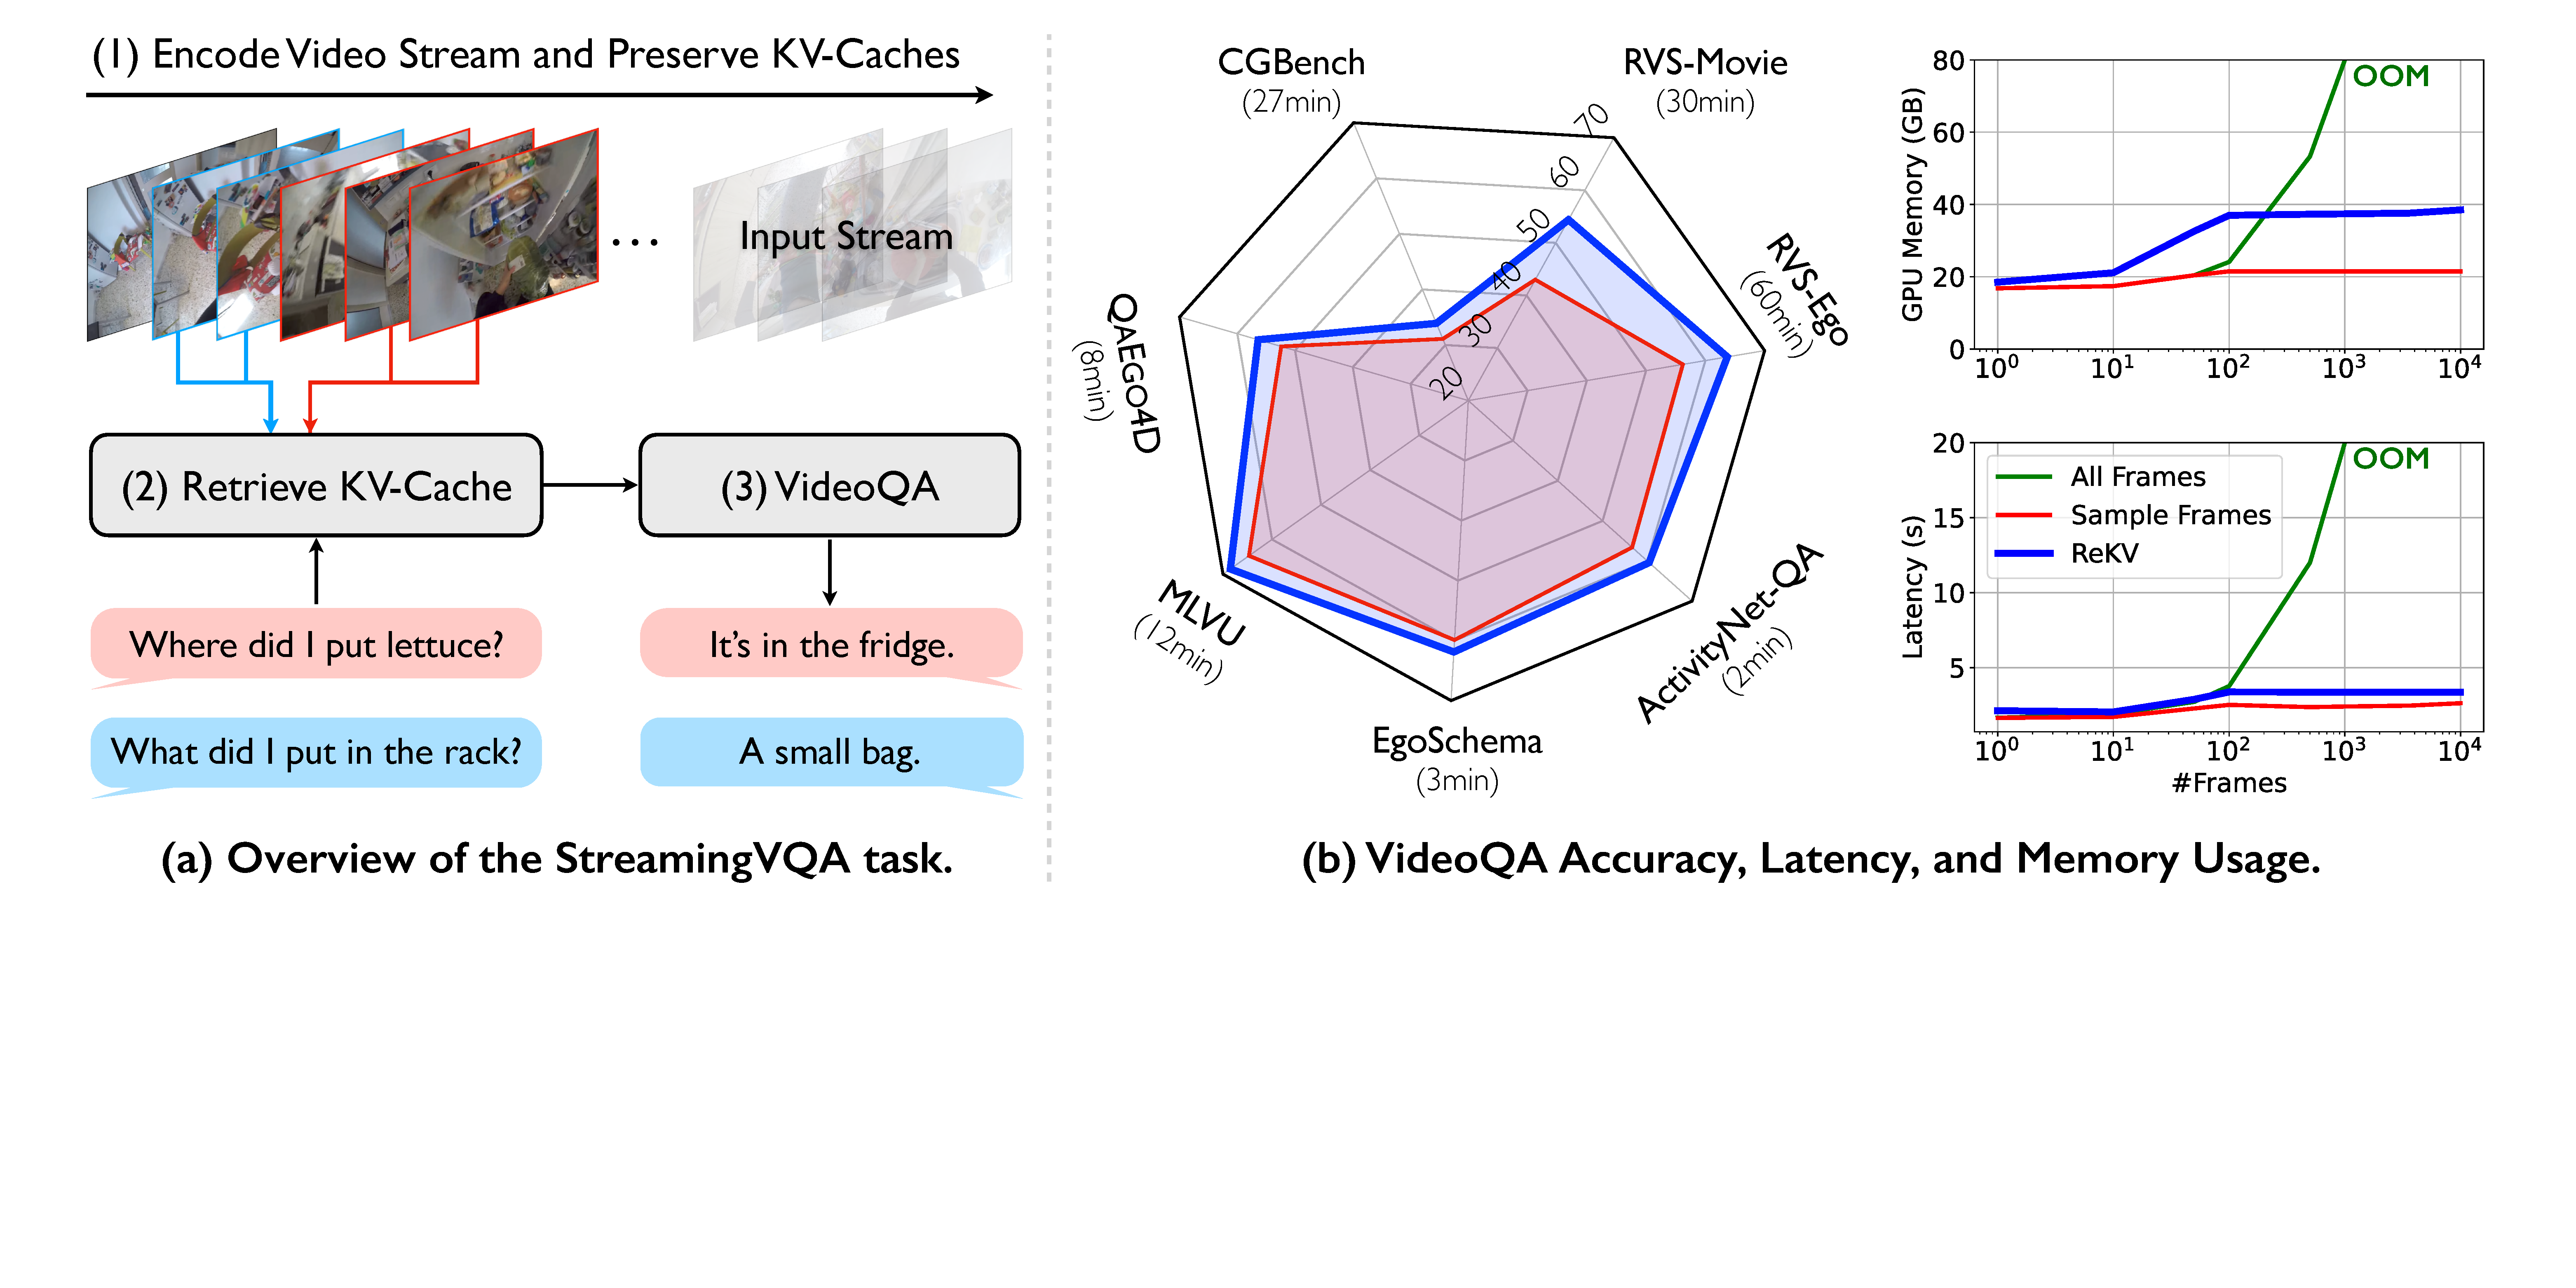
\includegraphics[height=\myfigheight, trim={0 0 415pt 0}, clip]{figures/teaser.pdf}
        \caption{\hermes Framework}
        \label{fig:teaser_a}
    \end{subfigure}
    % --- 子图 (b) ---
    \begin{subfigure}{\widthof{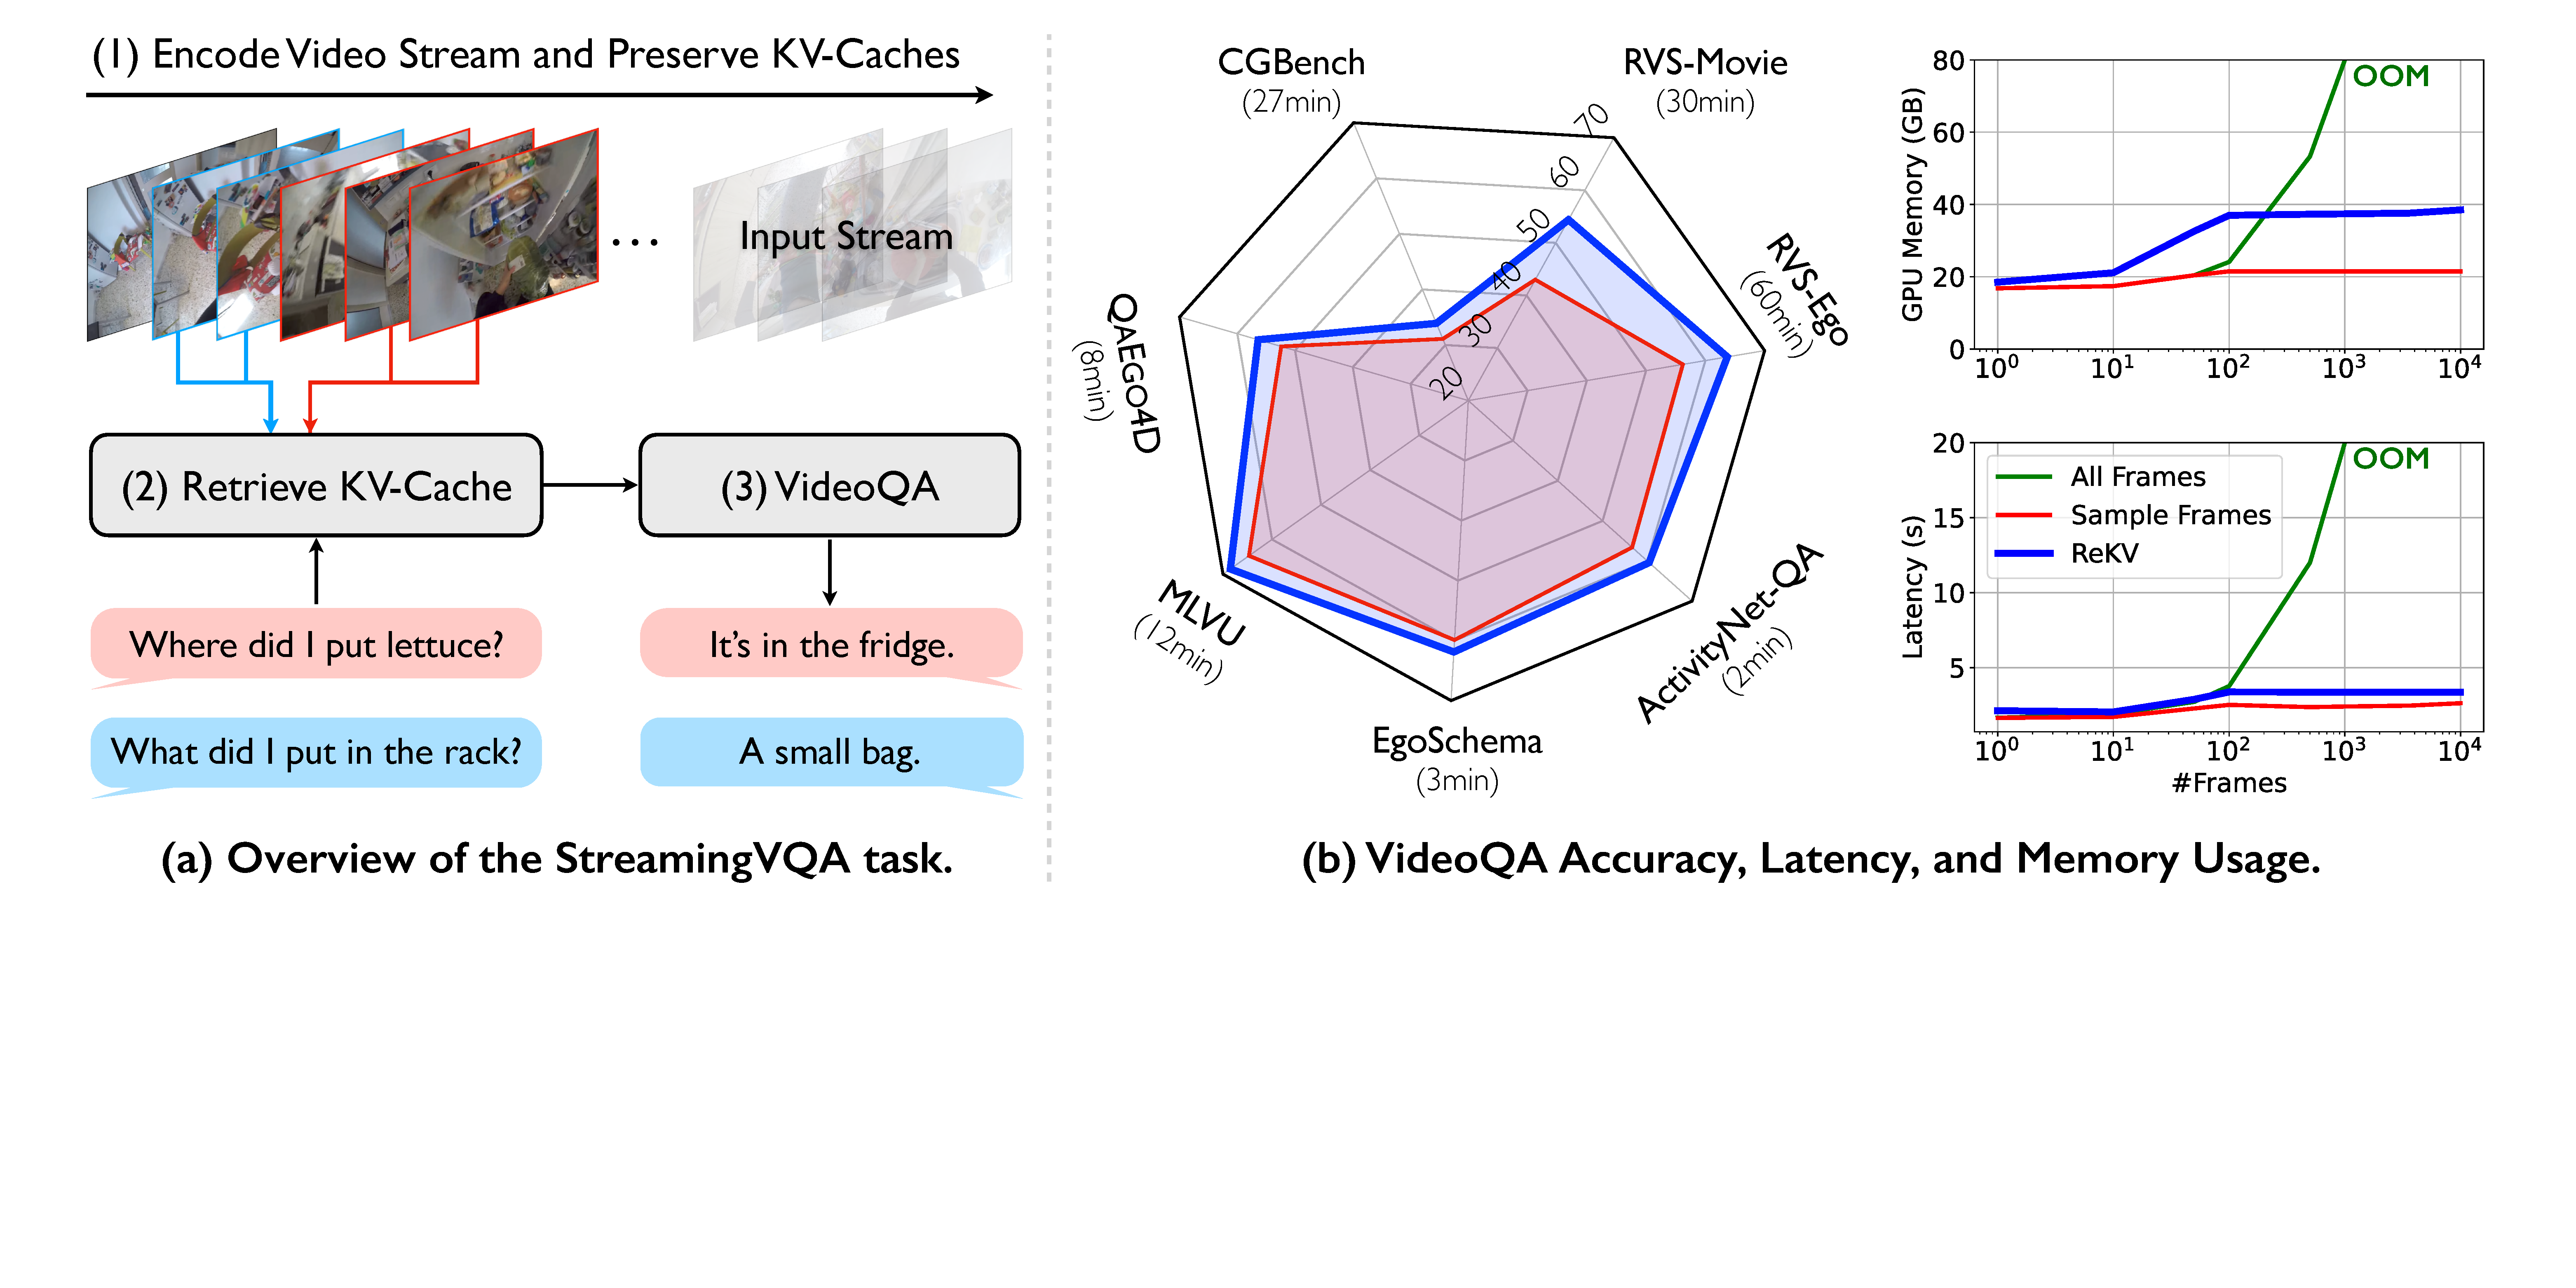
\includegraphics[height=\myfigheight, trim={365pt 0 251pt 0}, clip]{figures/teaser.pdf}}}
        \centering
        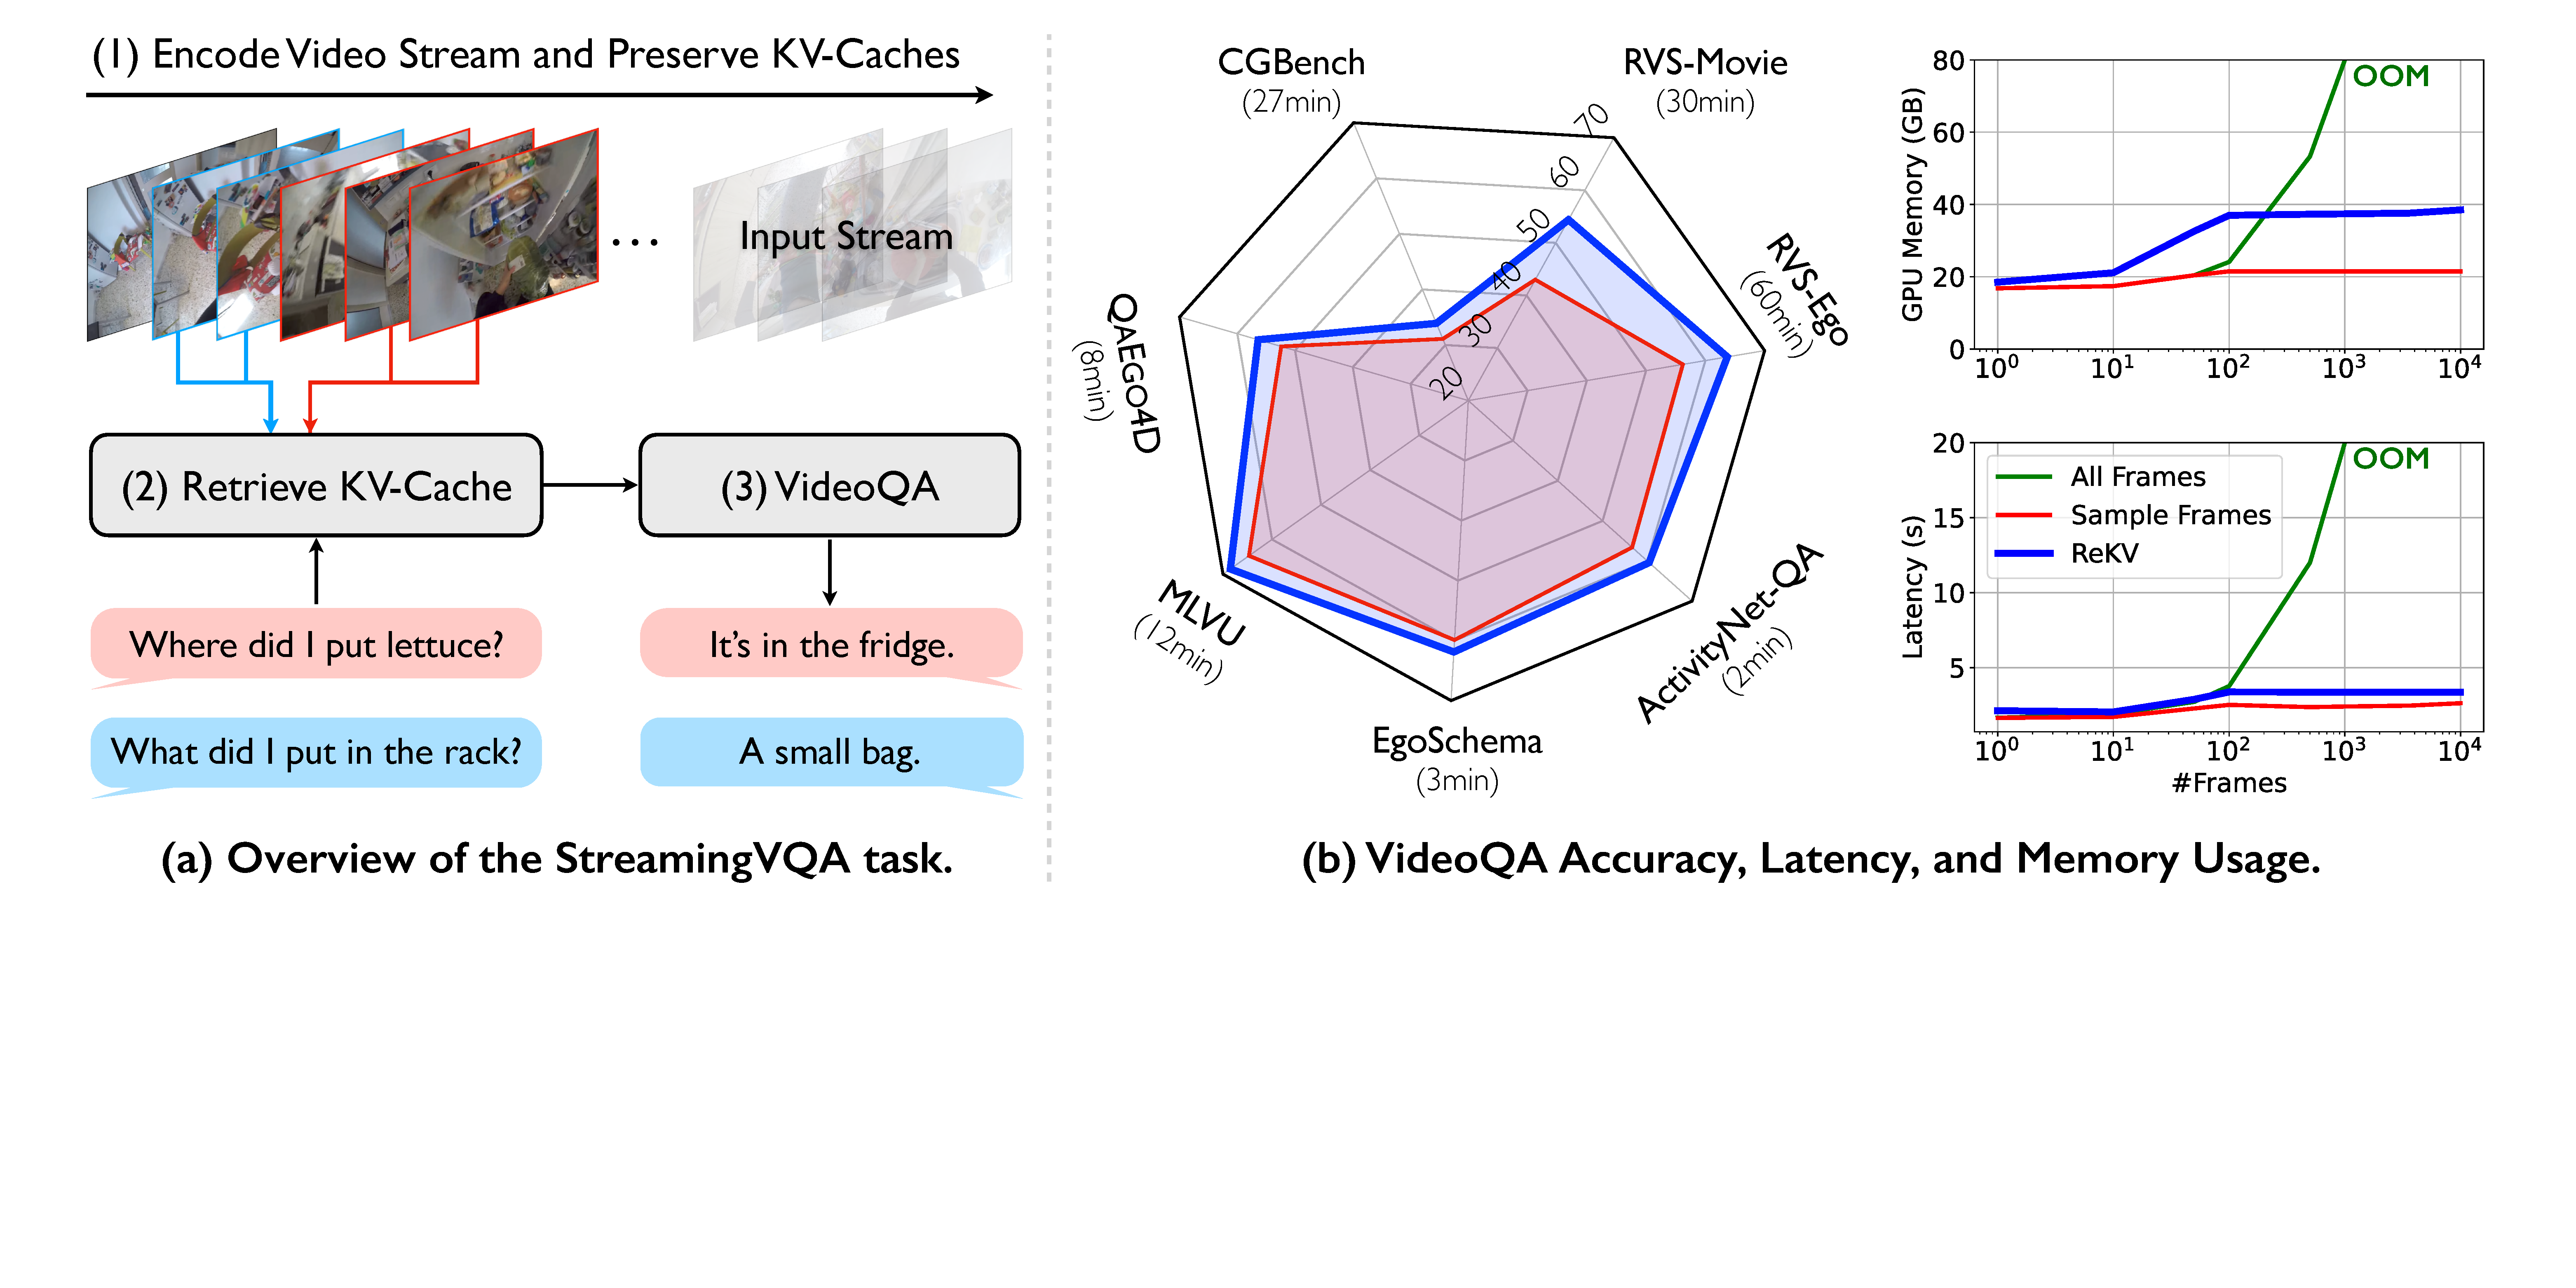
\includegraphics[height=\myfigheight, trim={365pt 0 251pt 0}, clip]{figures/teaser.pdf}
        \caption{Attention Analysis}
        \label{fig:teaser_b}
    \end{subfigure}
    % --- 子图 (c) ---
    \begin{subfigure}{\widthof{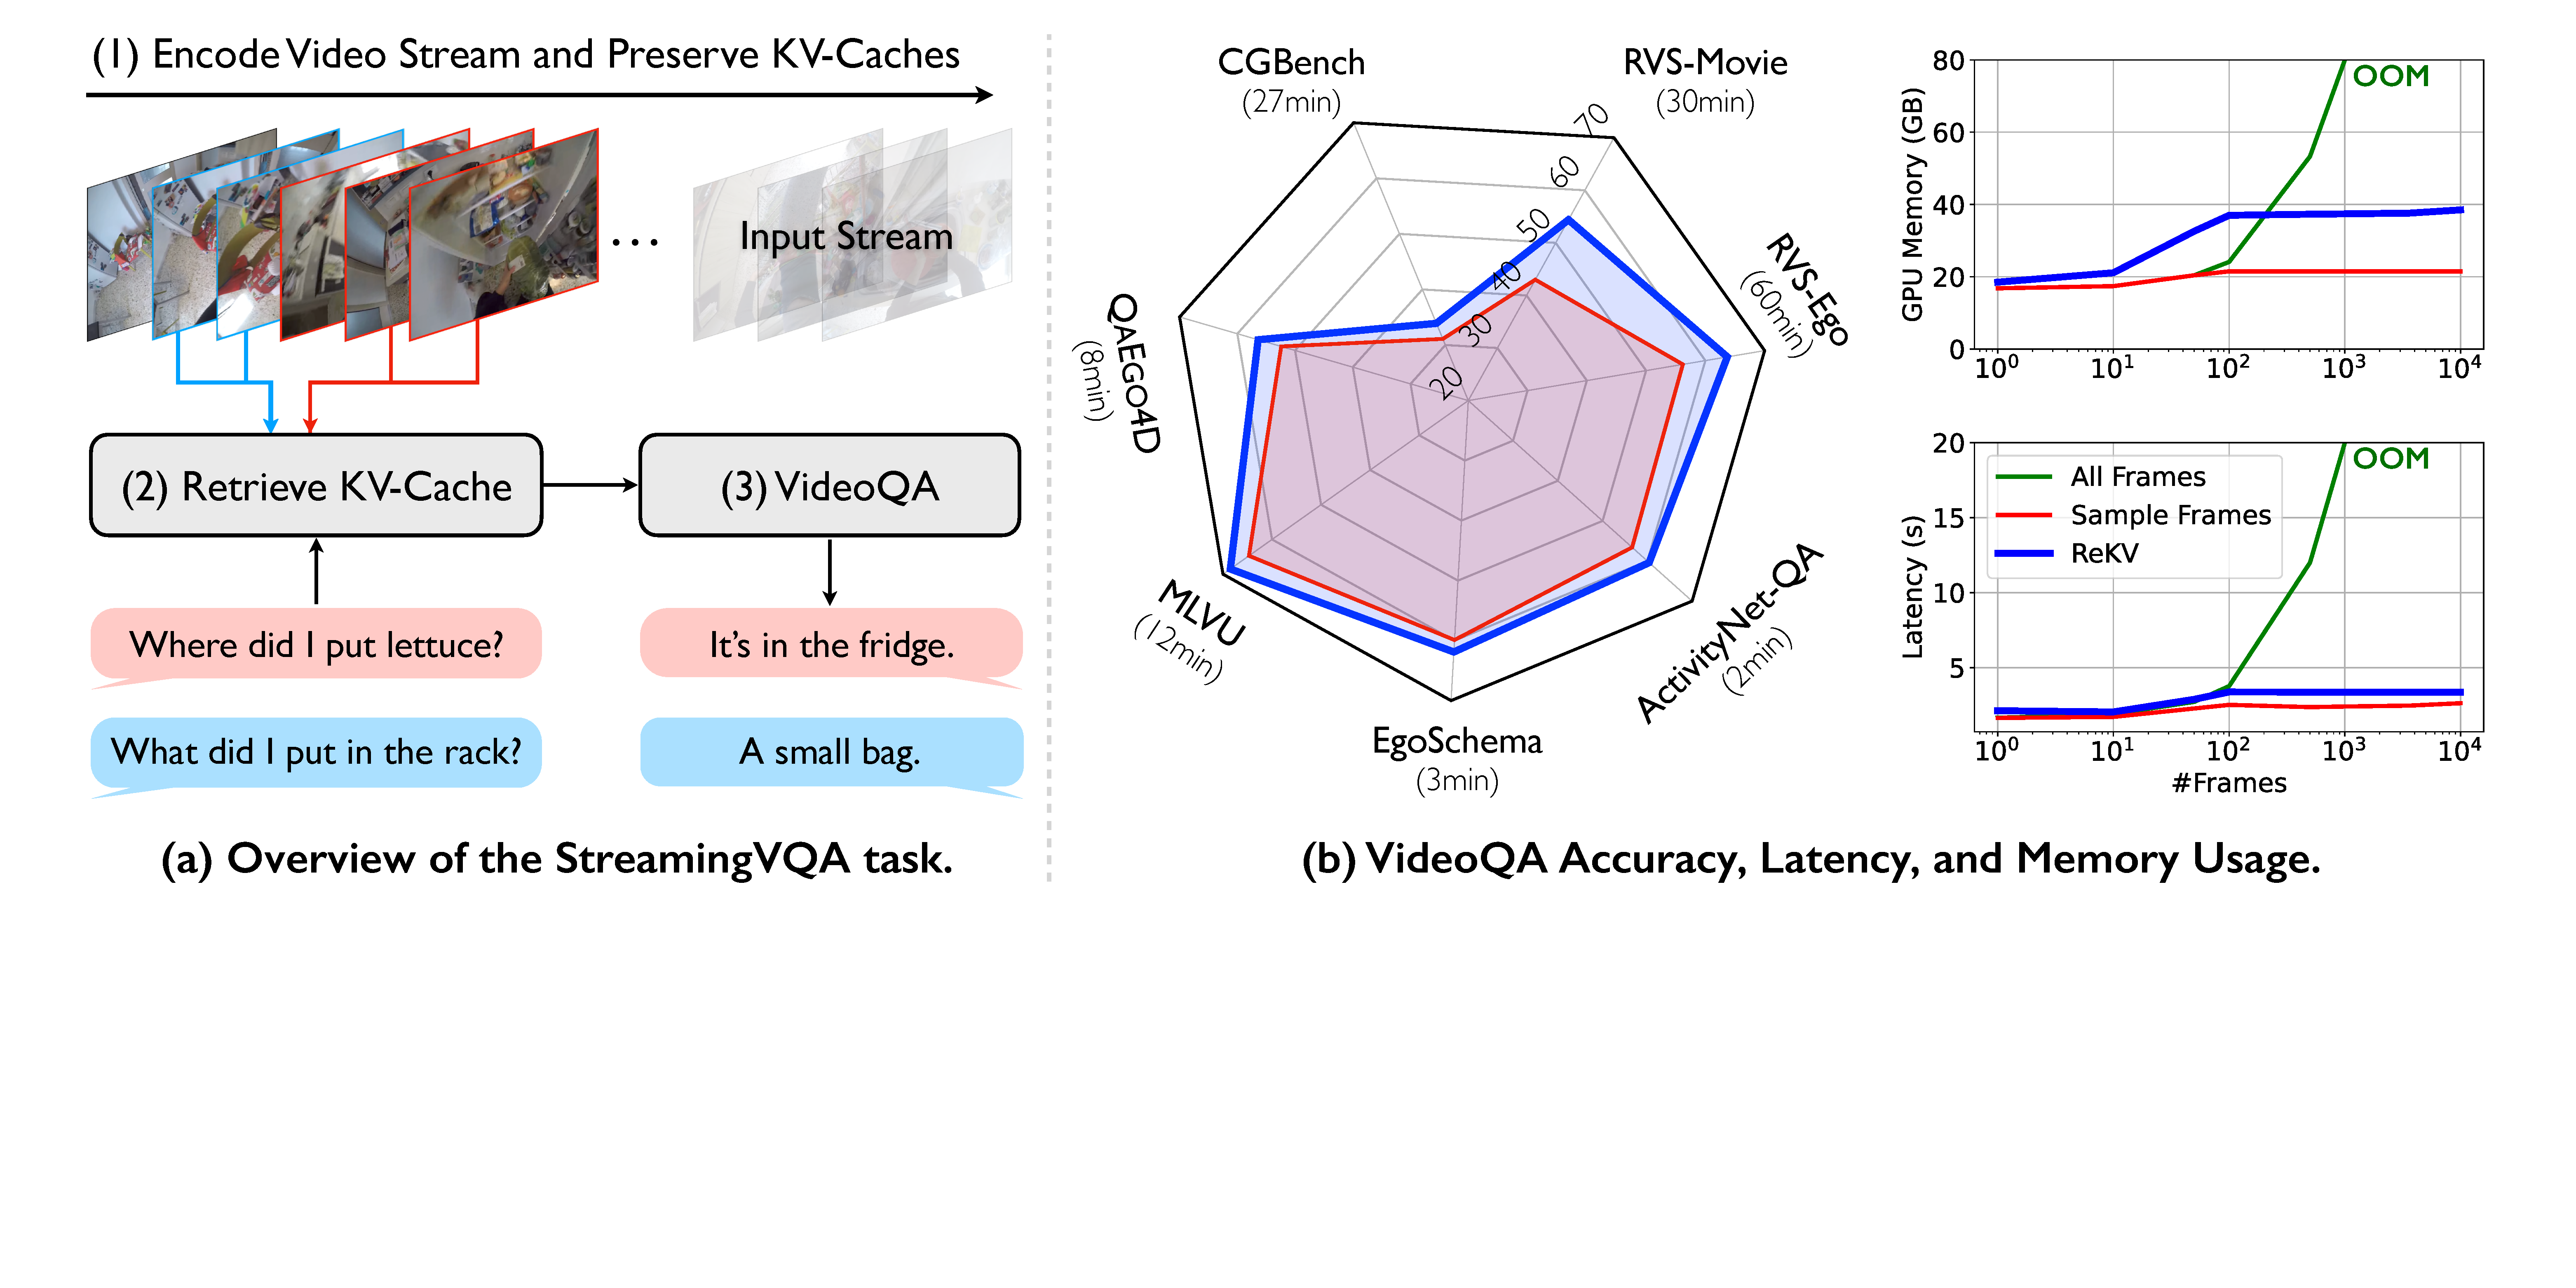
\includegraphics[height=\myfigheight, trim={529pt 0 0 0}, clip]{figures/teaser.pdf}}}
        \centering
        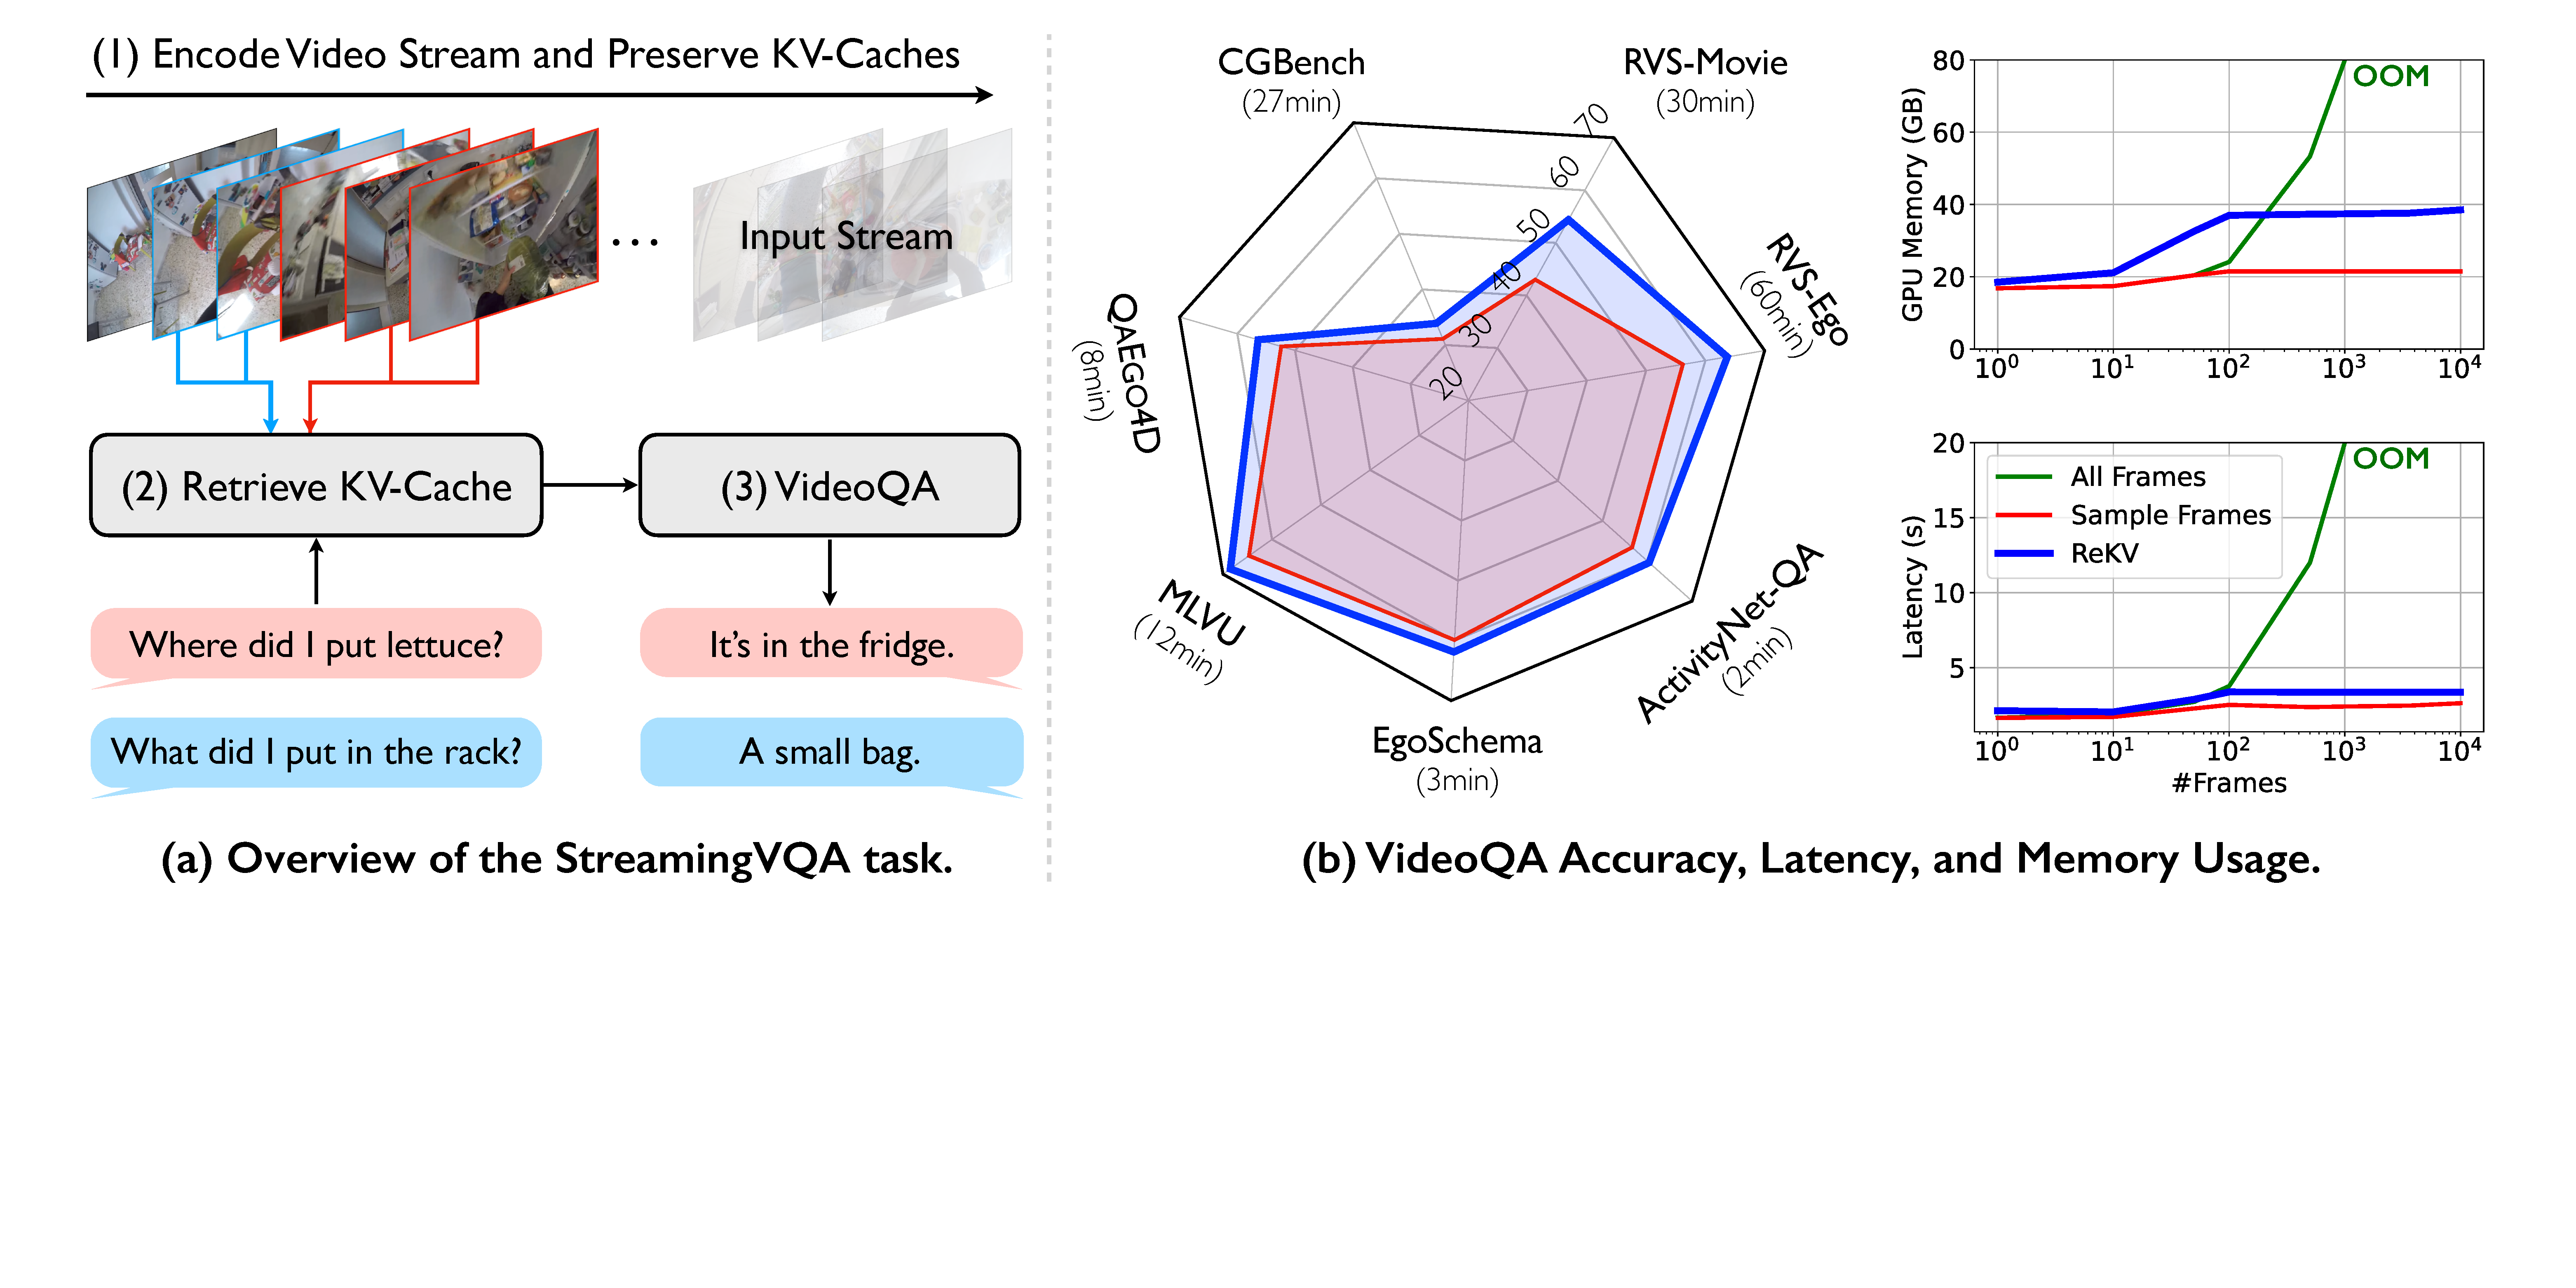
\includegraphics[height=\myfigheight, trim={529pt 0 0 0}, clip]{figures/teaser.pdf}
        \caption{Efficiency Test}
        \label{fig:teaser_c}
    \end{subfigure}
    \caption{\textbf{Left}: \hermes is a training-free approach for efficient streaming video understanding, enabling stable inference by reusing KV cache and performing hierarchical management of video tokens stored in KV cache. \textbf{Middle}: \hermes is based on a mechanistic investigation of the layer-wise attention preferences over hierarchical video information. \textbf{Right}: We evaluate \llava on a single A800 GPU (80 GB). As input frames increase, \hermes consistently maintains extremely low latency (TTFT < 30 ms) and stable GPU memory consumption, exhibiting no risk of OOM errors and requiring no auxiliary external computational resources.}
\end{figure*}



\section{Introduction}
\label{sec:introduction}

% 必须强调流式视频推理的三个重点:1. 稳定准确的推理性能(accuracy) 2. 实时响应 3. 方便端侧设备部署的低GPU memory usage

% 流式输入带来的新挑战

Recent years have witnessed remarkable evolution in the capabilities of Multimodal Large Language Models (MLLMs) in video understanding tasks~\cite{gemini25, li2024llavaonevisioneasyvisualtask, bai2025qwen3vltechnicalreport}.
% Specifically, these models have demonstrated comprehensive understanding and reasoning abilities across various temporal durations and diverse downstream tasks~\cite{li2024mvbenchcomprehensivemultimodalvideo, fu2025videommefirstevercomprehensiveevaluation, mangalam2023egoschemadiagnosticbenchmarklongform}.
Despite the progress, the rapid emergence of real-time applications demands stable long video understanding, low-latency response, and memory-efficient deployment. 
%Consequently, the research frontier is shifting from offline paradigms to streaming video understanding.
%has imposed rigorous demands on MLLMs regarding long temporal context understanding, low-latency inference, and memory efficiency. Consequently, the research frontier is shifting from traditional offline inference paradigms toward streaming inference capable of processing continuous video inputs.
% 现有的offline compression方法由于流式输入的特殊性,无法直接使用
However, existing MLLMs struggle to simultaneously satisfy these requirements on streaming videos.
% Some works streaming methods necessitate expensive model-specific training~\cite{wang2025streambridgeturningofflinevideo, xu2025streamingvlmrealtimeunderstandinginfinite, zeng2025streamforestefficientonlinevideo}, leaving training-free approaches relatively underexplored.
Notably, TimeChat-Online~\cite{timechatonline} observes that a large number of streaming video tokens are redundant, motivating compression methods to address these challenges. While numerous compression techniques have been proposed for offline videos~\cite{wang2025videotreeadaptivetreebasedvideo, yang2024visionziplongerbetternecessary, tao2025dycokedynamiccompressiontokens}, most are ill-suited for memory management in streaming scenarios, as streaming inputs are unpredictable in future frames and queries.
%posing significant challenges for prior static compression methods.
% 现有流式压缩方法的局限,主要有两点: 1. 依赖外挂式记忆和临时检索,时延高。内置式记忆探索得较少,将记忆能力内化入模型很重要 2. 很多是模型特定的训练方法,开销大,不够通用(相对training-free)

To adapt to streaming inputs, recent research introduces specialized memory management techniques, which generally fall into two paradigms: external memory and internal memory. External memory methods store video content as captions or raw vision patches in databases, and perform ad-hoc retrieval and multimodal prefilling at query time~\cite{xiong2025streamingvideounderstandingmultiround, yang2025streamagentanticipatoryagentsstreaming}, suffering from high latency and a lack of end-to-end cohesion. Additionally, many of these methods necessitate costly model-specific training~\cite{wang2025streambridgeturningofflinevideo, xu2025streamingvlmrealtimeunderstandinginfinite, zeng2025streamforestefficientonlinevideo}. In contrast, internalizing memory directly into the key-value cache (KV cache) remains underexplored, yet is crucial for low-latency responses and seamless end-to-end reasoning over stored video contexts. Moreover, KV cache naturally acts as a latent, model-intrinsic memory~\cite{hu2025memoryageaiagents} that frequently interacts with the video stream, making it particularly suitable for training-free memory management. ReKV~\cite{di2025streamingvideoquestionansweringincontext} and LiveVLM~\cite{ning2025livevlmefficientonlinevideo} are representative training-free, cache-based methods for streaming memory management. They store previous video segments in external CPU or disk and need to perform an additional retrieval when a user query arrives, which still rely on external computational resources and leads to significant latency. StreamMem~\cite{yang2025streammemqueryagnostickvcache} leverages chat template tokens to guide compression but lacks fine-grained KV management and mechanistic interpretability.%\jlfu{Discussing how our method differs from other KV-cache–based approaches (e.g., ReKV, StreamMem, and LiveVLM)}

% 正式介绍HERMES这个方法,顺带再提一个之前工作的不足:缺乏机制可解释性

To overcome the aforementioned limitations of existing streaming video methods, we propose \hermes (KV Cache as \underline{\textbf{H}}i\underline{\textbf{ER}}archical \underline{\textbf{M}}emory for \underline{\textbf{E}}fficient \underline{\textbf{S}}treaming Video Understanding), a training-free and plug-and-play approach that can be seamlessly integrated into existing MLLMs. %as shown in \cref{fig:teaser}. 
Grounded in a mechanistic investigation of layer-wise attention shown in~\cref{fig:teaser_b}, we conceptualize KV cache as a hierarchical memory framework that stores video information across multiple levels of granularity: 
%shallow layers as sensory memory, deep layers as long-term memory and middle layers as transitional working memory.
shallow layers function as sensory memory, exhibiting a strong recency bias toward newly arriving frames; deep layers act as long-term memory, focusing on frame-level rhythmic anchor tokens; and middle layers serve as transitional working memory that balances recency information with frame-level semantic representations.
Our method \hermes comprises three components: \emph{hierarchical KV cache management}, \emph{cross-layer memory smoothing}, and \emph{position re-indexing}. During inference, \hermes reuses the compact KV cache and requires no auxiliary computations or external devices upon the arrival of user queries, thereby guaranteeing real-time responses. Experiments show that \hermes maintains stable and accurate performance with up to 68\% fewer video tokens, while maintaining consistently low response latency and a constant GPU memory footprint.

% In contrast to many prior multimodal compression works that rely on heuristic techniques~\cite{kim2025infinipotvmemoryconstrainedkvcache, yang2025streammemqueryagnostickvcache, chen2025streamkvstreamingvideoquestionanswering}, which struggle with limited interpretability and reliability, our approach is based on a mechanistic investigation of layer-wise attention preference for hierarchical video information.

%Grounded in a mechanistic investigation of layer-wise attention preferences for hierarchical video tokens, we conceptualize the key-value cache (KV cache) as a hierarchical memory framework that stores video information across multiple levels of temporal granularity.

% We observe that the shallow, middle, and deep decoder layers of MLLMs correspond to the short-term, mid-term, and long-term memory of streaming video information, respectively.


% \begin{itemize} [leftmargin=*]
% \itemsep0em 
% \item 
% \textbf{Shallow Layers as Short-term Memory}: For the short-term video memory stored in the shallow layers, where attention exhibits a strong preference for temporally recent video tokens, we employ a First-In-First-Out (FIFO) eviction strategy to only keep the recent video tokens.
% \item
% \textbf{Middle Layers as Mid-term Memory}: The middle layers serve as a transition from short-term to long-term memory. These layers increasingly focus on video content that is temporally distant from the time point of user queries, with attention patterns becoming progressively sparser. Token eviction in this stage is determined by a weighted combination of attention and recency scores of video tokens. To account for unpredictable user queries, we utilize specifically designed local and global guidance prompts to steer the compression.
% \item
% \textbf{Deep Layers as Long-term Memory}: In the deep layers, attention is extremely sparse, and the bias toward recent video tokens largely disappears. These layers primarily capture global and abstract semantic information. Compression is guided by attention scores from the global guidance prompt. To maximize the preservation of video information, evicted tokens are aggregated into a summary token maintained at the end of the sequence.
% \end{itemize}

%Beyond the hierarchical design, we introduce \emph{layer consistency} as a smoothing mechanism. This allows the long-term memory in deeper layers to provide feedback for token retention in earlier layers, thereby mitigating information inconsistencies across different memory stages. 

% Finally, to support potentially infinite video streams, especially in resource-limited scenarios, we maintain a fixed and compact GPU memory footprint at all times. We implement a \emph{soft position encoding reassignment} method to ensure both stable comprehension performance and an enhanced perception of recent temporal dynamics, which are essential for streaming understanding~\cite{xu2025streamingvlmrealtimeunderstandinginfinite}.


To summarize, our main contributions are as follows:
\begin{enumerate}[leftmargin=*]
\itemsep0em 
\item
Grounded in a mechanistic analysis on attention visualization, we pioneer the conceptualization of KV cache as a hierarchical video memory framework across multiple granularities.

\item
We propose \hermes, a training-free method for streaming video understanding by reusing hierarchically managed KV cache. Despite reducing video tokens by up to 68\%, \hermes achieves competitive accuracy, with gains of up to 11.4\% on streaming benchmarks.

\item
\hermes exhibits outstanding efficiency in streaming scenarios. Compared to the prior training-free SOTA method, it achieves up to a 10$\times$ speedup in latency. With a constant, compact GPU memory footprint and no auxiliary computation at query time, \hermes ensures consistently low-latency responses.

\end{enumerate}

\section{StreamingVQA: Task Definition and Discussion} 
\label{sec:task}

This paper considers the problem of streaming video question-answering (\textbf{StreamingVQA}), where a model continuously processes a video stream and can respond to questions about past visual content at any moment. 
In this section, we formally define the task and outline the design principles for our proposed solution.

Given a video stream $\mathcal{V}^T := [v_1, v_2, ..., v_T]$ consisting of $T$ frames and a set of $N$ questions $\mathcal{Q} := \{q_1, q_2, \dots, q_N\}$,
StreamingVQA aims to answer a question $q_i$ at any time step $t~(1 \le t \le T)$, using only the frames seen up to that point, $\mathcal{V}^t := [v_1, v_2, ..., v_t]$.


\noindent\textbf{Discussion-I: StreamingVQA {\em vs.}~OfflineVQA.} StreamingVQA involves continuously analyzing an incoming video stream and answering questions based on the observed visual content at any moment. 
In contrast, conventional video question-answering models~\citep{frozen_bilm,video_chatgpt,llava_next_video,llava_onevision} operate in an offline mode, referred to as OfflineVQA.
The two paradigms differ in that: 
1) StreamingVQA processes a continuous video stream, while OfflineVQA handles a predefined video input, and 
2) StreamingVQA allows questions to be asked at any point during the stream, whereas OfflineVQA processes questions only after the entire video has been viewed.
Notably, OfflineVQA can be considered a special case of StreamingVQA, where all questions are posed after the video is fully processed. 


Conventional approaches typically employ a visual encoder~\citep{clip,siglip,fang2023eva} and a projection module~\citep{llava_next_video,blip2} to process video frames~($\mathcal{V}^t$).
The output is concatenated with the tokenized question to form a sequence $[\mathcal{V}_t, q_i]$~\footnote{We maintain the original notation for simplicity.}, which is then passed to an LLMs to predict an answer.
However, this approach is impractical due to the high computational cost associated with processing a large number of frames ($T$).


A common workaround is sparse frame sampling~\citep{video_chatgpt, llava_next_video, llava_onevision}, 
but this introduces new problems:
(i) loss of critical visual information, leading to incomplete or inaccurate responses, and
(ii) the need to reprocess frames for different questions, since questions asked at different time points require distinct frame samples. This becomes increasingly inefficient as $T$ and $N$ grow.

Given these challenges, current OfflineVQA methods fall short when applied to StreamingVQA scenarios. Therefore, designing a new approach optimized for StreamingVQA is crucial to handling video streams more efficiently, enabling real-time question answering and unlocking more interactive video analysis applications.


\noindent\textbf{Discussion-II: Design Principles for Efficient StreamingVQA.} 
To tackle the aforementioned challenges, we can exploit the causal nature of the LLM decoder to avoid redundant computations and strike a balance between accuracy and speed. 
During attention calculations, causal masking prevents the model from accessing future tokens, ensuring that video tokens are encoded independently of the questions. This allows us to \textit{decouple video encoding from question-answering}.

For video encoding, we leverage the KV-Cache optimization to accelerate inference.
However, as number of frames grows large, handling the massive number of video tokens becomes increasingly inefficient and may exceed the model’s capacity~\citep{lm_infinite,streamingllm}.
To address this, we adopt a sliding-window attention mechanism~\citep{lm_infinite}, which limits the attention scope to only the most recent frames.

Regarding question-answering, Video KV-Caches are stored and can be reused as context to answer different questions. 
However, long video sequences produce a substantial amount of KV-Caches, leading to excessive GPU memory consumption, computational overhead, and unnecessary distractions if all are used.
To address this, we introduce an efficient retrieval method that selects the most relevant video key-value vectors from the video KV-Caches. These selected vectors then serve as context, enabling efficient and scalable StreamingVQA.




\section{
\ourmethod: \underline{Re}trieve In-context Video \underline{KV}-Cache
}
\label{sec:method}

This section introduces \textbf{\ourmethod}, an approach that integrates seamlessly with a Video-LLM to enable efficient StreamingVQA without requiring additional training.
Overall, \ourmethod~efficiently encodes the video stream, maintains its KV-Caches, retrieves relevant caches based on the given question, and uses them for accurate question-answering.

\begin{figure}[t]
\centerline{\includegraphics[width=.85\linewidth]{figures/src/framework.pdf}}
\caption{
\textbf{Overview of~\ourmethod.}
We modify the attention mechanism in Decoder-based Video-LLMs:
(a) The video stream is encoded with sliding-window attention (Equation~\ref{equ:video_encoding}), with out-of-window Video KV-Caches offloaded to RAM or disk.
(b) Upon receiving a question, relevant key-value vectors are retrieved based on cosine similarity, with compressed vectors to accelerate retrieval (Equation~\ref{equ:retrieval}).
(c) The retrieved key-value vectors are reloaded onto the GPU and utilized for autoregressive answer generation (Equation~\ref{equ:answer_generation}).
}
\label{fig:framework} 
\end{figure}

We aim to enable Video-LLMs, trained on limited frames, 
to perform StreamingVQA \textbf{without additional training}.
As shown in Figure~\ref{fig:framework}, 
the proposed \ourmethod~has three components: 
video stream encoding, video KV-Cache retrieval, and question-answering using the retrieved key-value vectors.

\noindent\textbf{Video Stream Encoding with Sliding-window Attention.} 
We encode the video stream $\mathcal{V}^T$ incrementally, processing it chunk by chunk.
At each step, the inputs include past key-value vectors $\mathbf{P} = \{(\mathbf{k}_j, \mathbf{v}_j)\}_{j=1}^{l_P}$ and the current tokens $\mathbf{X}=\{\mathbf{t}_{i+l_P}\}_{i=1}^{l_X}$, 
where $l_P$ denotes the lengths of past key-values, and $l_X$ refers to the chunk size.
The local key-value vectors within a window $l_L$ can thus be derived as 
$\mathbf{L} = \mathbf{P}_{[l_P - l_L + 1 : l_P]}$.
The attention calculation is then formulated as:
\begin{equation}
    \mathbf{O} = \text{Attn}\left(\mathbf{W_Q}\mathbf{X}, [\mathbf{L}_k, \mathbf{W_K}\mathbf{X}], [\mathbf{L}_v, \mathbf{W_V}\mathbf{X}]\right),
    \label{equ:video_encoding}
\end{equation}
where $\mathbf{W_Q}$, $\mathbf{W_K}$, and $\mathbf{W_V}$ are the attention layer parameters, $\mathbf{L}_k$ and $\mathbf{L}_v$ correspond to the key and value vectors in $\mathbf{L}$. All video KV-Caches are stored for future retrieval. For extremely long videos, we manage memory constraints by offloading KV-Caches to RAM or disk, as in~\citep{infllm}.

\noindent\textbf{External Video KV-Cache Retrieval.} 
Here, we utilize an external CLIP-like model~\citep{clip, siglip} to retrieve question-relevant video KV-Cache, primarily as a baseline to assess whether retrieval can enhance VideoQA performance, as demonstrated in Section~\ref{sec:experiments}. 
Specifically, a CLIP-like model transformers each video frame into a vector $\mathbf{v} = f_v(v) \in \mathrm{R}^D$, where $f_v$ represents the visual encoder, $D$ denotes the vector dimension. Similarly, the question is encoded as $\mathbf{q} = f_t(q) \in \mathrm{R}^D$, where $f_t$ is the text encoder. We then compute the cosine similarity between the embeddings of frame and question: 
\begin{equation}
    \text{Sim}(\mathbf{v}, \mathbf{q}) = \frac{\mathbf{v} \cdot \mathbf{q}}{\tau~||\mathbf{v}||~||\mathbf{q}||}
    \label{equ:retrieval}
\end{equation} 
where $\tau$ is a learnable temperature parameter. This similarity is calculated at the frame level, rather than at the token level. Alternatively, we can group $b$ consecutive frames into blocks by averaging their frame vectors and then compute block-level similarity scores. Finally, the $r$ most relevant video frames or $\lceil r/b \rceil$ video blocks are retrieved. The corresponding video KV-Cache, denoted as $\mathbf{R}$, is subsequently loaded onto the GPU for question-answering.

\noindent\textbf{Internal Video KV-Cache Retrieval.} Building on recent advancements in handling long sequences with LLMs~\citep{infllm, quickllama, em_llm}, we further explore using self-attention layers within Video-LLMs for retrieval. Similar to external retrieval, internal retrieval is still performed at the level of video frames or blocks.

During video modeling, the average of the key vectors of a frame is computed as its representative frame vector: $\mathbf{v} = \frac{1}{N_f} \sum_{j=1}^{N_f} \mathbf{k}_j \in \mathrm{R}^{D'}$, where $N_f$ is the number of tokens per frame, and $\mathbf{k}_j$ is the $j$-th key vector. 
To reduce computational overhead, we do not differentiate between attention heads and instead concatenate them into a single vector, with $D'$ as the resultant dimension. Similarly, the question vector is computed as $\mathbf{q} = \frac{1}{N_q} \sum_{k=1}^{N_q} \mathbf{q}_{k} \in \mathrm{R}^{D'}$, where $N_q$ is the number of tokens in the question, 
and $\mathbf{q}_{k}$ is its $k$-th query vector. The similarity computation and video KV-Cache retrieval are identical to that of external retrieval, except that $\tau$ is set to 1.

Note that, internal retrieval offers several advantages over external retrieval. 
First, it operates independently within each self-attention layer, allowing different layers to retrieve different video blocks.\footnote{For simplicity, we omit the layer index in the above explanation.}
This allows for a broader capture of video context. 
Additionally, internal retrieval reuses already computed hidden representations and does not introduce extra parameters, which reduces the computational overhead compared to external retrieval.

\noindent\textbf{Question-Answering Using Retrieved KV.} The retrieved Video KV-Caches serve as the context for video question-answering. Formally, the attention calculation is formulated as:
\begin{equation}
    \mathbf{O} = \text{Attn}\left(\mathbf{W_Q}\mathbf{X}, [\mathbf{R}_k, \mathbf{W_K}\mathbf{X}], [\mathbf{R}_v, \mathbf{W_V}\mathbf{X}]\right),
    \label{equ:answer_generation}
\end{equation} 
where $\mathbf{X}$ represents either the question tokens or the current token being decoded, and $\mathbf{R}_k$ and $\mathbf{R}_v$ are the key and value vectors from the context, which includes the retrieved video, question, and previously generated tokens. 

\noindent\textbf{Positional Encoding.}
Our baseline Video-LLMs employ Rotary Position Embeddings (RoPE)~\citep{su2024roformer}, a commonly used relative positional encoding method.
Our video streaming encoding process follows LM-Infinite~\citep{lm_infinite}, where RoPE operates normally within the local window but is constrained by a ``distance ceiling'' for more distant tokens. 
For question-answering, we do not account for the original positions of the retrieved KV-Caches, as handling unseen distances among tokens presents significant challenges~\citep{lm_infinite}.
Instead, we treat these retrieved tokens as regular consecutive tokens. 
We also experimented with a static variation from Inf-LLM~\citep{infllm}, where all retrieved tokens are assigned the same position. 
Our results show that applying standard RoPE to retrieved video tokens leads to better performance, likely due to the importance of capturing temporal information in video comprehension.

\section{Experiments}
\label{sec:experiments}

\subsection{Experimental Setup}
\paragraph{Benchmarks.}
We evaluate \hermes on diverse streaming and offline benchmarks. For streaming understanding, we use StreamingBench~\cite{lin2024streamingbenchassessinggapmllms}, OVO-Bench~\cite{li2025ovobenchfarvideollmsrealworld} and RVS (including RVS-Ego and EVS-Movie)~\cite{zhang2024flashvstreammemorybasedrealtimeunderstanding}.
%These benchmarks follow the streaming video QA paradigm, limiting the available visual context to only the video content before the current timestamp. Additionally, unpredictable user questions occur at any time.
For offline video evaluation, we adopt one short video dataset MVBench~\cite{li2024mvbenchcomprehensivemultimodalvideo}, along with two long video datasets, VideoMME~\cite{fu2025videommefirstevercomprehensiveevaluation} and Egoschema~\cite{mangalam2023egoschemadiagnosticbenchmarklongform}. We conduct evaluation on the official dev split of Egoschema and report VideoMME results without subtitles. Our benchmark selection covers both multiple-choice and open-ended questions as QA form. The details of utilized benchmarks are demonstrated in~\cref{app:details_of_benchmarks}.

\paragraph{Models.}
To further verify the broad applicability of our method, we select two popular open-source MLLM series, LLaVA-OneVision (LLaVA-OV)~\cite{li2024llavaonevisioneasyvisualtask} and Qwen2.5-VL~\cite{bai2025qwen25vltechnicalreport}. Each is tested across two different parameter scales, covering a large range from 0.5B to 32B. For Qwen2.5-VL, we maintain its native dynamic resolution on video input, ensuring a fair comparison with the base model.

\paragraph{Implementation Details.}
For evaluating \hermes across all benchmarks, each video is encoded and processed chunk by chunk, with 16 frames per chunk, and sequentially prefilling the backbone LLM. Then, token compression is triggered once the predefined memory budget is exceeded.

For the layer partition, we follow the mechanistic investigations presented in ~\cref{sec: investigation}: 10\% shallow, 60\% middle and 30\% deep layers. A more comprehensive analysis of attention behaviors as supportive evidence can be found in~\cref{fig:more_vis}. The cross-layer memory smoothing hyperparameter $\lambda$ proposed in~\cref{sec: smoothing} is layer-dependent, with detailed configurations reported in~\cref{app:smooth_config}.


All evaluations are conducted using FP16 mixed precision and efficiency tests are conducted on a single A800 GPU, consistent with prior works~\cite{di2025streamingvideoquestionansweringincontext, chen2025streamingtomstreamingtokencompression}. Greedy decoding is used to generate deterministic outputs. Accuracy evaluations can be completed on one H200 GPU.

\subsection{Main Results}
\paragraph{Streaming Video Understanding}
\begin{table*}[ht]
\renewcommand{\arraystretch}{0.9}
% \renewcommand\tabcolsep{4.3pt}
    \centering
    \footnotesize
    % 6 columns: Model, Frames, StreamingBench, OVO-Bench-rt, OVO-Bench-backward, OVO-Bench-Avg.
    % \resizebox{0.98\linewidth}{!}{
    \begin{tabular}{l c | c c c c}
    \toprule
    \multirow{2}{*}{\textbf{Model}} & \multirow{2}{*}{\textbf{\#Frames}} & \textbf{StreamingBench} & \multicolumn{3}{c}{\textbf{OVO-Bench}} \\
    & & Real-Time & Real-Time & Backward & \textbf{Avg.} \\
    \midrule
    \midrule
    Human & - & 91.46 & 93.20 & 92.33 & 92.83 \\
    \midrule
    \multicolumn{6}{c}{\textbf{Proprietary MLLMs}} \\
    \midrule
    Gemini 1.5 pro~\cite{gemini25} & 1 fps & 75.69 & 69.32 & 62.54 & 66.41\\
    GPT-4o~\cite{openai2024gpt4ocard} & 64 & 73.28 & 64.46 & 60.75 & 62.87\\
    Claude 3.5 Sonnet~\cite{claude3_5} & 20 & 72.44 & - & - & -\\
    \midrule
    \multicolumn{6}{c}{\textbf{Open-source Offline MLLMs}} \\
    \midrule
    Video-LLaMA2-7B~\cite{videollama2} & 32 & 49.52 & - & - & -\\
    VILA-1.5-8B~\cite{vila} & 14 & 52.32 & - & - & -\\
    Video-CCAM-14B~\cite{videoccam} & 96 & 53.96 & - & - & -\\
    LongVA-7B~\cite{longva} & 128 & 59.96 & - & - & -\\
    Qwen2-VL-7B~\cite{wang2024qwen2vlenhancingvisionlanguagemodels} & 64 & 69.04 & 60.65 & 48.58 & 54.62 \\
    InternVL-V2-8B~\cite{internvl2} & 16 & 63.72 & 60.73 & 44.00 & 52.37 \\
    % Kangaroo-7B~\cite{kangaroo} & 64 & 64.60 & - & - & -\\
    LLaVA-NeXT-Video-32B~\cite{llava-next} & 64 & 66.96 & - & - & -\\
    MiniCPM-V-2.6-8B~\cite{minicpm} & 32 & 67.44 & - & - & -\\
    \addlinespace[1pt]
    
    \midrule
    \multicolumn{6}{c}{\textbf{Open-source  Online MLLMs}} \\
    \midrule
    Flash-VStream-7B~\cite{flashvstream} & - & 23.23 & 29.86 & 25.35 & 27.61\\
    VideoLLM-online-8B~\cite{videollmonline} & 2 fps & 35.99 & 20.79 & 17.73 & 19.26\\
    Dispider-7B~\cite{dispider} & 1 fps & 67.63 & 54.55 & 36.06 & 45.31\\
    TimeChat-Online-7B~\cite{timechatonline} & 1 fps & 75.36 & 61.90 & 41.70 & 51.80\\
    StreamForest-7B~\cite{zeng2025streamforestefficientonlinevideo} & 1 fps & 77.26 & 61.20 & 52.02 & 56.61 \\

    \midrule
    \multicolumn{6}{c}{\textbf{Training-free Offline-to-Online Methods}} \\
    \midrule
    LLaVA-OV-7B~\cite{li2024llavaonevisioneasyvisualtask} & 64 & 71.34 & 63.06 & 43.64 & 53.35 \\

    \hspace{3pt} + ReKV~\cite{di2025streamingvideoquestionansweringincontext} & 0.5 fps &  69.22 & 57.33 & 44.16 & 50.75 \\

    \hspace{3pt} + LiveVLM~\cite{ning2025livevlmefficientonlinevideo} & 0.5 fps & 72.92 & - & - & -\\

    \hspace{3pt} + StreamKV~\cite{chen2025streamkvstreamingvideoquestionanswering} & 0.5 fps & 68.80 & - & - & -\\

    \rowcolor{gray!20}  \hspace{3pt} + HERMES (6K tokens) & 0.5 fps & 72.63 & 65.07 & 48.80 & 56.94 \\

    \rowcolor{gray!40}  \hspace{3pt} + HERMES (4K tokens) & 0.5 fps & \textbf{73.23} & \textbf{66.34} & \textbf{50.20} & \textbf{58.27} \\
    
    \midrule

    LLaVA-OV-0.5B~\cite{li2024llavaonevisioneasyvisualtask} & 64 & 59.64 & 49.70 & 34.59 & 42.15 \\

    \hspace{3pt} + ReKV~\cite{di2025streamingvideoquestionansweringincontext} & 0.5 fps &  57.39 & 43.77 & 33.06 & 38.42 \\

    \rowcolor{gray!20} \hspace{3pt} + HERMES (6K tokens) & 0.5 fps & 61.04 & 50.34 & 34.75 & 42.55 \\

     \rowcolor{gray!40} \hspace{3pt} + HERMES (4K tokens) & 0.5 fps & \textbf{62.04} & \textbf{50.72} & \textbf{34.80} & \textbf{42.76} \\
    
    \midrule    
    Qwen2.5-VL-7B~\cite{bai2025qwen25vltechnicalreport} & 1 fps & 73.31 & 59.90 & 44.65 & 52.28 \\
    \rowcolor{gray!20} \hspace{3pt} + HERMES (6K tokens) & 1 fps & 78.72 & 68.42 & 48.10 & 58.26 \\
    \rowcolor{gray!40}\hspace{3pt} + HERMES (4K tokens) & 1 fps & \textbf{79.44} & \textbf{68.98} & \textbf{49.43} & \textbf{59.21} \\
    
    \midrule
    
    Qwen2.5-VL-32B~\cite{bai2025qwen25vltechnicalreport} & 1 fps & 74.27 & 64.40 & 50.33 & 57.37 \\
    \rowcolor{gray!20}\hspace{3pt} + HERMES (6K tokens) & 1 fps & \textbf{80.20} & 71.93 & \textbf{57.71} & \textbf{64.82} \\
    \rowcolor{gray!40}\hspace{3pt} + HERMES (4K tokens) & 1 fps & 80.08 & \textbf{72.37} & 55.42 & 63.90 \\

    
    \bottomrule
    
    \end{tabular}
    \caption{Performance comparison (\%) on StreamingBench and OVO-Bench. The "Avg." column reports the results of the average accuracy of real-time visual perception and backward tracing tasks.}
    \label{tab:streaming_main}
\end{table*}



\begin{table}[t]
    \centering
    \begin{minipage}[t]{0.49\textwidth}
      \centering
      \small
      \resizebox{\linewidth}{!}{
      \begin{tabular}{lcccc}
        \toprule
        \multirow{2}{*}{\textbf{Model}} & \multicolumn{2}{c}{\textbf{RVS-Ego}} & \multicolumn{2}{c}{\textbf{RVS-Movie}} \\
        \cmidrule(lr){2-3} \cmidrule(lr){4-5}
         & \textbf{Acc} & \textbf{Score} & \textbf{Acc} & \textbf{Score} \\
        \midrule
        \llava~\cite{li2024llavaonevisioneasyvisualtask} & 56.2 & 3.7 & 43.0 & 3.3 \\
        \hspace{3pt}+ ReKV$^{\dag}$ \citep{di2025streamingvideoquestionansweringincontext} & 63.7 & 4.0 & 54.4 & 3.6  \\
        \hspace{3pt}+ ReKV w/o off.~\cite{di2025streamingvideoquestionansweringincontext} & 55.8 & 3.3 & 50.8 & 3.4 \\
        \hspace{3pt}+ Flash-VStream \citep{flashvstream} & 57.0 & 4.0 & 53.1 & 3.3 \\
        \hspace{3pt}+ InfiniPot-V \citep{kim2025infinipotvmemoryconstrainedkvcache} & 57.9 & 3.5 & 51.4 & 3.5 \\
        \hspace{3pt}+ StreamMem \citep{yang2025streammemqueryagnostickvcache} & 57.6 & 3.8 & 52.7 & 3.4 \\
        \hspace{3pt}+ StreamingTOM~\cite{chen2025streamingtomstreamingtokencompression} & 58.3 & 3.9 & 53.2 & 3.5 \\
        \rowcolor{gray!20}\hspace{3pt}+ HERMES (6K tokens) & \textbf{60.3} & \textbf{4.0} & \textbf{54.4} & \textbf{3.6} \\
        \rowcolor{gray!40}\hspace{3pt}+ HERMES (4K tokens) & 58.3 & 3.9 & \textbf{54.4} & \textbf{3.6} \\
        \midrule
        
        \llavasmall~\cite{li2024llavaonevisioneasyvisualtask} & 51.8 & 3.7 & 37.2 & 3.2 \\
        \hspace{3pt}+ ReKV$^{\dag}$ \citep{di2025streamingvideoquestionansweringincontext} & 54.7 & 3.9 & 44.6 & 3.4  \\
        \rowcolor{gray!20}\hspace{3pt}+ HERMES (6K tokens) & \textbf{53.0} & \textbf{3.8} & \textbf{42.5} & \textbf{3.4} \\
        \rowcolor{gray!40}\hspace{3pt}+ HERMES (4K tokens) & 52.7 & 3.8 & 41.7 & \textbf{3.4} \\
        \bottomrule
        
      \end{tabular}
      }
      \caption{Performance on RVS-Ego and RVS-Movie. \dag: ReKV caches the KV states of all previously seen frames and is therefore treated as an upper bound.}
      \label{tab:rvs}
    \end{minipage}%
    \hfill%
    \begin{minipage}[t]{0.49\textwidth}
        \centering
        \small
        \resizebox{\linewidth}{!}{
        \begin{tabular}{l cccc}
        \toprule
        \multirow{2}{*}{\textbf{Metric}} & \multicolumn{4}{c}{\textbf{Frames}} \\
        %\cmidrule(lr){2-5}
         & \textbf{16} & \textbf{64} & \textbf{256} & \textbf{512}\\
        \midrule
        \multicolumn{5}{c}{\textit{\textbf{Chunk Size: 8}}} \\
        GPU Mem. / GB $\downarrow$          & 16.54 & 16.66 & 16.66 & 16.66  \\
        TTFT / ms $\downarrow$               & 27.01 & 28.41 & 28.44 & 28.41  \\
        TPOT / ms $\downarrow$  & 24.43 & 23.89 & 24.02 & 23.98 \\
        \midrule
        \multicolumn{5}{c}{\textit{\textbf{Chunk Size: 16}}} \\
        GPU Mem. / GB $\downarrow$          & 17.46 & 17.66 & 17.66 & 17.66 \\
        TTFT / ms $\downarrow$               & 27.02 & 28.97 & 28.50 & 28.38 \\
        TPOT / ms $\downarrow$  & 24.50 & 23.59 & 23.56 & 23.63 \\
        \bottomrule
        \end{tabular}
        }
        \caption{Efficiency across input frame numbers under two chunk sizes. "TTFT" denotes \textit{Time to First Token} and "TPOT" denotes \textit{Time Per Output Token}.}
        \label{tab:efficiency_chunk}
    \end{minipage}
\end{table}

Extensive experiments on streaming benchmarks reveal the key findings: 

\noindent
(1) \textit{\hermes outperforms on multiple-choice streaming datasets, showing exceptional real-time understanding and backward tracing capabilities}.
As shown in~\cref{tab:streaming_main}, it achieves state-of-the-art performance on StreamingBench and OVO-Bench, significantly surpassing base models and training-free baselines. Built on \qwen, \hermes reaches 79.44\% and 59.21\% accuracy using only 4K video tokens, improving over \qwen by 6.13\% and 6.93\%, while outperforming all 7B-scale open-source online and offline models. Full results on StreamingBench and OVO-Bench are shown in~\cref{tab:streamingbench_full} and~\cref{tab:ovobench_full} respectively.


\noindent
(2) \textit{\hermes excels on open-ended streaming tasks, showing fine-grained temporal and spatial comprehension}. On RVS-Ego and RVS-Movie (\cref{tab:rvs}), we evaluate the model answer by GPT-3.5-turbo-0125 on accuracy and score (1–5 scale), consistent with compared baselines.
\hermes consistently surpasses all prior training-free methods and improves accuracy by up to 11.4\% over the base model with uniformly sampled 64 frames. These extensive experiments demonstrate \hermes's strong abilities in various streaming tasks, as well as its general applicability across foundation models. Moreover, we provide case studies from RVS benchmark, showing finer-grained temporal (shown in~\cref{fig:case_temporal}) and spatial understanding (shown in ~\cref{fig:case_spatial}) abilities of \hermes than its base model.

\paragraph{Offline Video Understanding}
\begin{table}[t]
    \centering
    %\scriptsize
    %\small
    % 6 columns: Model, Frames, VideoMME (long), VideoMME (Avg), Egoschema, MVBench.
    \begin{tabular}{l c | c c c c}
    \toprule
    \multirow{2}{*}{\textbf{Model}} & \multirow{2}{*}{\textbf{\#Frames}} & \textbf{MVBench} & \textbf{Egoschema} & \multicolumn{2}{c}{\textbf{VideoMME}} \\
    % 
    & & & & Long & \textbf{Avg.} \\
    \midrule
    \midrule

    \multicolumn{6}{c}{\textbf{Proprietary MLLMs}} \\
    \midrule
    Gemini 1.5 pro~\cite{gemini25} & 1 fps & 75.69 & 69.32 & 62.54 & 66.41\\
    GPT-4o~\cite{openai2024gpt4ocard} & 64 & 73.28 & 64.46 & 60.75 & 62.87\\
    Claude 3.5 Sonnet~\cite{claude3_5} & 20 & 72.44 & - & - & -\\
    \midrule
    \multicolumn{6}{c}{\textbf{Open-source Offline MLLMs}} \\
    \midrule
    Video-LLaMA2-7B~\cite{videollama2} & 32 & 49.52 & - & - & -\\
    VILA-1.5-8B~\cite{vila} & 14 & 52.32 & - & - & -\\
    Video-CCAM-14B~\cite{videoccam} & 96 & 53.96 & - & - & -\\
    LongVA-7B~\cite{longva} & 128 & 59.96 & - & - & -\\
    LLaVA-Video-7B~\cite{zhang2025llavavideovideoinstructiontuning} & 32 & 58.60 & 57.3 & - & 63.30 \\
    Qwen2-VL-7B~\cite{wang2024qwen2vlenhancingvisionlanguagemodels} & 64 & 67.00 & 66.70 & - & 63.30 \\
    InternVL-V2-8B~\cite{internvl2} & 16 & 65.80 & - & - & 56.30 \\
    Kangaroo-7B~\cite{kangaroo} & 64 & 64.60 & - & - & -\\
    LLaVA-NeXT-Video-32B~\cite{llava-next} & 64 & 66.96 & - & - & -\\
    MiniCPM-V-2.6-8B~\cite{minicpm} & 32 & 67.44 & - & - & -\\
    
    
    \addlinespace[1pt]
    
    \midrule
    \multicolumn{6}{c}{\textbf{Open-source  Online MLLMs}} \\
    \midrule
    Dispider-7B~\cite{dispider} & 1 fps & - & 55.60 & - & 57.20\\
    TimeChat-Online-7B~\cite{timechatonline} & 1 fps & 75.36 & 61.90 & 41.70 & 53.22\\
    StreamForest-7B~\cite{zeng2025streamforestefficientonlinevideo} & 1 fps & 70.20 & - & - & 61.40\\
    \midrule
    \multicolumn{6}{c}{\textbf{Training-free Offline-to-Online Methods}} \\
    \midrule
    LLaVA-OV-7B~\cite{li2024llavaonevisioneasyvisualtask} & 64 & \textbf{57.02} & 59.93 & 48.00 & 57.67 \\

    \hspace{3pt} + ReKV~\cite{di2025streamingvideoquestionansweringincontext} & 0.5 fps &  56.83 & \textbf{60.70} & 46.89 & 57.74 \\

    \rowcolor{gray!20}  \hspace{3pt} + HERMES (6K tokens) & 0.5 fps & 56.95 & 60.23 & 49.11 & 58.44 \\

     \rowcolor{gray!40}  \hspace{3pt} + HERMES (4K tokens) & 0.5 fps & 56.92 & 60.29 & \textbf{49.22} & \textbf{58.85} \\
    
    \midrule    
    Qwen2.5-VL-7B~\cite{bai2025qwen25vltechnicalreport} & 1 fps & 65.00 & 58.47 & 53.89 & \textbf{64.52}\\
    \rowcolor{gray!20}\hspace{3pt} + HERMES (6K tokens) & 1 fps & 65.40 & 59.47 & \textbf{54.44} & 62.00 \\
    \rowcolor{gray!40} \hspace{3pt} + HERMES (4K tokens) & 1 fps & \textbf{65.53} & \textbf{59.97} & 53.44 & 60.63 \\
    
    
    \bottomrule
    \end{tabular}
    \vspace{-6pt}
    \caption{Performance comparison (\%) on offline benchmarks.}
    \label{tab:offline_main}
\end{table}



The results presented in~\cref{tab:offline_main} demonstrate the \textit{competitive performance of \hermes across multiple temporal scales on offline benchmarks}, compared to the base model and other training-free methods. Under a limited budget of video tokens, \hermes achieves performance that is better than or comparable to the corresponding base models. \hermes based on \llava surpasses the base model on long video datasets Egoschema and VideoMME, achieving 60.29\% and 58.85\%, respectively, and attains 56.92\% accuracy on the short video dataset MVBench, which is comparable to the base model's 57.02\%.


\subsection{Efficiency Analysis}
\begin{figure}[ht]
  \centering
    \includegraphics[width=\linewidth]{figures/efficiency_compare_new.pdf}
    %\vspace{-6pt}
  \caption{GPU memory and TTFT latency comparison across input frame numbers. \hermes achieves 10 $\times$ faster in TTFT compared to prior SOTA.}
  \label{fig:efficency_compare}
\end{figure}



To evaluate the efficiency of \hermes, we utilize three metrics: peak GPU memory usage, Time to First Token (TTFT), defined as the latency measured from the moment a user inputs a query to the decoding of the first output token, and Time Per Output Token (TPOT) across varying numbers of input frames. All experiments are conducted using \llava as the base model with a 4K-token memory budget. ~\cref{fig:efficency_compare} shows the comparison of memory usage and TTFT among \hermes and representative streaming methods. Unlike Dispider and LiveVLM, \hermes consistently maintains stable memory usage and TTFT as frames increase. Notably, under the 256-frame setting, \hermes achieves 1.04$\times$ reduction in peak memory compared to the prior SOTA LiveVLM, while achieving an impressive 10$\times$ speedup in TTFT over the prior SOTA StreamingTOM.

We further examine the efficiency of \hermes under varying encoded video chunk sizes, with the results shown in~\cref{tab:efficiency_chunk}. GPU memory usage does not increase with longer video lengths due to the fixed memory budget. TTFT and TPOT remain consistently low across varying video lengths and encoding chunk sizes, confirming real-time responsiveness in practical streaming scenarios.


\subsection{Ablation Study}

We conduct ablation studies to evaluate the contributions of \hermes's components and hyperparameter choices, covering: (1) KV cache memory budget, (2) cross-layer memory smoothing and its hyperparameters, (3) position re-indexing strategies for streaming and offline datasets, and (4) summary tokens for long-term memory retention.

\paragraph{Memory Budget}
\label{sec:memory_ablation}
% \begin{figure}[ht]
%   \centering
%     \includegraphics[width=0.95\linewidth]{figures/llava_budget_ablation.pdf}
%     \caption{Performance comparison of \llava across different memory budgets.}
%   \label{fig:memory_ablation_llava}
% \end{figure}
\begin{figure}[ht]
\begin{subfigure}[ht]{0.47\linewidth}
    \centering
    \includegraphics[width=\linewidth]{figures/llava_budget_ablation.pdf}
    \caption{Performance comparison of \llava across different memory budgets.}
    \label{fig:memory_budget_llava}
  \end{subfigure}
  \quad
  \begin{subfigure}[ht]{0.47\linewidth}
    \centering
    \includegraphics[width=\linewidth]{figures/qwen_budget_ablation.pdf}
    \caption{Performance Comparison of \qwen across Different Memory Budgets.}
    \label{fig:memory_budget_qwen}
  \end{subfigure}
\end{figure}



To investigate the impact of  memory budget on understanding performance, we conduct ablations by varying the memory budget $|M|$ from 1K to 10K. As shown in~\cref{fig:memory_budget_llava}, for \hermes built upon LLaVA-OV-7B, the performance on both streaming and offline datasets stabilizes once memory budget reaches 4K. Notably, streaming datasets can tolerate a smaller memory budget. In contrast, the performance on long offline datasets degrades significantly when the memory budget is below 4K. The ablation on \qwen is provided in~\cref{fig:memory_budget_qwen}, yielding conclusions consistent with those on \llava.%Therefore, to balance the performance and efficiency, we choose to report the performance with a memory budget of 4K and 6K in main results.

\begin{table}[t]
    \centering
    \begin{minipage}[t]{0.47\textwidth}
    \centering
    \small
    \resizebox{\linewidth}{!}{
    \begin{tabular}{ccc | cccc}
        \toprule
         \multicolumn{3}{c|}{\textbf{Hyperparameter}} & \multicolumn{4}{c}{\textbf{VideoMME}} \\
        %\cmidrule(lr){1-3} \cmidrule(lr){4-7}
        %\midrule
        $\lambda_{deep}$ & $\lambda_{mid}$ & $\lambda_{shallow}$ & Short & Medium & Long & \textbf{Avg.}\\
        \midrule
        0 & 0 & 0   & 69.67 & 51.11 & 43.44 & 54.74 \\
        0.5 & 0 & 0   & 69.67 & 51.44 & 43.56 & 54.89 \\
        0 & 0.5 & 0   & 70.89 & 54.78 & 46.44 & 57.37 \\
        0 & 0 & 0.5   & 70.89 & 54.44 & 47.00 & 57.44 \\
        0.5 & 0.5 & 0.5   & \textbf{71.78} & 54.78 & 47.33 & 57.96 \\
        \rowcolor{gray!40}0.4 & 0.3 & 0.1   & 71.33 & \textbf{54.89} & \textbf{49.11} & \textbf{58.44} \\
        \bottomrule
    \end{tabular}
    }
    \caption{Ablation on different cross-layer memory smoothing hyperparameter $\lambda$.}
    \label{tab:lambda_ablation}
    \end{minipage}
    \quad
    \begin{minipage}[t]{0.47\textwidth}
        \centering
        \small
        \resizebox{\linewidth}{!}{
        \begin{tabular}{lc|cccc}
        \toprule
         \multirow{2}{*}{\textbf{Model}} & \multirow{2}{*}{\textbf{Aggregation}} & \multicolumn{4}{c}{\textbf{VideoMME}} \\
        %\cmidrule(lr){3-6}
        & & Short & Medium & Long & \textbf{Avg.}\\
        \midrule
        \llava & - & 69.89 & 55.11 & 48.00 & 57.67 \\
        \hspace{3pt}+ HERMES & w/o & 71.33 & 54.78 & 47.78 & 57.96 \\
        \rowcolor{gray!40} \hspace{3pt}+ HERMES & w/ & \textbf{71.33} & 54.89 & \textbf{49.11} & \textbf{58.44} \\
        \bottomrule
    \end{tabular}
    }
    
    \caption{Ablation on summary tokens in deep layers. The gray row is our default setting in all experiments.}
    \label{tab:summary_token_ablation}
    \end{minipage}
\end{table}
\paragraph{Cross-Layer Memory Smoothing}
In~\cref{tab:lambda_ablation}, we evaluate variants without the proposed cross-layer memory smoothing mechanism, as well as alternative hyperparameter configurations. All these variants exhibit degraded performance on the VideoMME benchmark, demonstrating both the critical role of memory smoothing and the effectiveness of our chosen hyperparameter settings.


\begin{table}[ht]
    \centering
    \begin{minipage}[t]{0.47\textwidth}
        \centering
        \small
        \resizebox{\linewidth}{!}{
        \begin{tabular}{lc|c|ccc}
        \toprule
         \multirow{2}{*}{\textbf{Model}} & \multirow{2}{*}{\textbf{Re-Indexing}} & \textbf{StrBench} & \multicolumn{3}{c}{\textbf{OVO-Bench}} \\
        %\cmidrule(lr){4-6}
        & & Real-Time & Real-Time & Backward & \textbf{Avg.}\\
        \midrule
        \llava & - & 71.34 & 63.06 & 43.64 & 53.35 \\
        \rowcolor{gray!40} \hspace{3pt}+ HERMES & lazy & \textbf{72.63} & \textbf{65.07} & \textbf{48.80} & \textbf{56.94} \\
        \hspace{3pt}+ HERMES & eager & 72.30 & 64.91 & 47.21 & 56.06 \\
        \bottomrule
        \end{tabular}
        }
        \caption{Ablation on different re-indexing strategies on streaming benchmarks. The gray row represents our default setting in all evaluations for streaming benchmarks. "StrBench" represents \textit{StreamingBench}.}
        \label{tab:pos_ablation_streaming}
    \end{minipage}%
    \quad
    \begin{minipage}[t]{0.47\textwidth}
        \centering
        \small
        \resizebox{\linewidth}{!}{
        \begin{tabular}{lc|cccc}
        \toprule
         \multirow{2}{*}{\textbf{Model}} & \multirow{2}{*}{\textbf{Re-Indexing}} & \multicolumn{4}{c}{\textbf{VideoMME}} \\
        %\cmidrule(lr){3-6}
        & & Short & Medium & Long & \textbf{Avg.}\\
        \midrule
        \llava & - & 69.89 & 55.11 & 48.00 & 57.67 \\
        \hspace{3pt}+ HERMES & lazy & 69.67 & 51.67 & 43.44 & 54.93 \\
        \rowcolor{gray!40} \hspace{3pt}+ HERMES & eager & \textbf{71.33} & 54.89 & \textbf{49.11} & \textbf{58.44} \\
        \bottomrule
        \end{tabular}
        }
        \caption{Ablation on different re-indexing strategies on offline benchmark VideoMME. The gray row represents our default setting in all evaluations for offline benchmarks.}
        \label{tab:pos_ablation_offline}
    \end{minipage}
\end{table}
\paragraph{Position Re-Indexing Strategies}
For all streaming evaluations, we adopt the lazy position re-indexing strategy, while we use the eager re-indexing strategy for offline evaluations. Ablation studies in~\cref{tab:pos_ablation_streaming} and~\cref{tab:pos_ablation_offline} show the effectiveness of these strategies in their respective scenarios.

\paragraph{Summary Tokens in Deep Layers}
%\input{tables/summary_token_ablation}
In~\cref{sec: smoothing}, we aggregate the evicted tokens in each deep layer into one summary token at each compression step. The results in~\cref{tab:summary_token_ablation} indicate that these summary tokens effectively preserve long-term memory, leading to improved performance on VideoMME.
\section{Related Work}
\label{sec:related_work}

\noindent\textbf{LLMs for Video Understanding.} 
In recent years, there has been a surge of interest in leveraging Large Language Models (LLMs) for video understanding, leading to the development of several innovative approaches~\citep{video_chatgpt, llava_next_video, llava_onevision}. These models typically use a Vision Encoder to extract video features, followed by a mapping step with Linear Projection, MLP, or Q-Former~\citep{blip2}. The mapped features are combined with textual data and fed into large language models (LLMs) to generate a text output. These models have relatively simple architectures, requiring less training data and computational resources, yet they achieve strong performance on short video understanding benchmarks~\citep{msrvtt_qa, next_qa, li2024mvbench}. However, they employ sparse sampling or token compression techniques to reduce the number of tokens, which can result in significant information loss when dealing with longer or more content-rich videos. As a result, they are not well-suited for long video understanding or streaming video understanding.

\noindent\textbf{Long Video Understanding.} 
A central challenge in long video understanding is effectively compressing the information from lengthy videos. Many approaches use language as a bridge, condensing videos into dense captions~\citep{llovi,video_recap,streaming_dvc}. While this achieves good results in some cases, compressing video content into text often leads to the loss of crucial visual details. Besides, as a pioneering approach to streaming video understanding, VideoLLM-Online~\citep{videollm_online} employs a data-centric methodology by interleaving video and text during training. In contrast, our approach is training-free, allowing seamless integration with various existing Video-LLMs to extend their StreamingVQA capabilities. Additionally, VideoLLM-Online retains only a single token per frame to handle long videos, which may result in visual information loss. Our method preserves complete visual information and leverages In-Context KV-Cache Retrieval to enhance efficiency.

Another line of research focuses on compressing long videos into a memory bank~\citep{wu2019long, wu2022memvit, wang2023memory}.
MC-ViT~\citep{mc_vit} adapts existing pretrained video transformers by fine-tuning them to attend to condensed visual memories. It relates closely to the token-pruning, merging, and memory-based video understanding methods. In comparison, we propose a training-free method specifically tailored to the StreamingVQA task. Incorporating MC-ViT into the StreamingVQA task could be an interesting avenue for future research, and we acknowledge its potential in this domain.
This approach has been integrated into Video-LLMs for streaming video understanding, as shown in works like VideoStreaming~\citep{videostreaming} and Flash-VStream~\citep{flashvstream}. These methods dynamically update the memory during video processing and utilize it for downstream tasks.
Despite their innovation, a major limitation of these methods is their failure to account for video length and information density, especially when using a fixed memory size. For example, Flash-VStream compresses both 10-second clips and hour-long videos into the same 681 tokens.
Furthermore, these methods lack interpretability, making it difficult to determine how much information is being compressed into the memory or whether relevant video information is being accurately retrieved during downstream tasks.

In pursuit of greater interpretability in long video understanding, methods such as GroundVQA~\citep{di2023groundvqa} and GeLM~\citep{chen2024groundedmultihopvideoqalongform} advocate for localizing relevant video clips while responding to user queries. Drawing inspiration from these, this work refrains from excessively condensing video information. By harnessing the causal capabilities of Video-LLMs, it preserves the entire Video KV-Cache, allowing for the retrieval of relevant information when required. This strategy effectively mitigates the substantial loss of video content while improving interpretability.

\noindent\textbf{Long Context Handling for LLMs.} 
Handling long text sequences in LLMs has been a major challenge due to high computational and memory costs, leading to training constraints on shorter sequences.
Techniques like StreamingLLM~\citep{streamingllm} and LM-Infinite~\citep{lm_infinite} use sliding window attention to process long sequences incrementally, but discard distant tokens, limiting the model’s ability to capture long-range dependencies. Recent approaches~\citep{infllm,quickllama,em_llm} address this by storing and retrieving previously computed KV-Caches, enabling better recall of distant contexts.

\noindent\textbf{Retrieval-Augmented Generation.} 
Retrieval-augmented generation (RAG) combines retrieval mechanisms with generative models to enhance performance across various NLP tasks by incorporating external knowledge~\citep{guu2020retrieval,lewis2020retrieval,borgeaud2022improving} and improving performance in vision-language tasks~\citep{xu2024retrieval}. In-context retrieval, recently proposed for handling long inputs~\citep{ram2023context}, retrieves information from the input document itself rather than an external knowledge base. In-context KV-Cache retrieval further improves efficiency by pre-encoding long documents, avoiding redundant encodings, and leveraging the LLM’s own retrieval capabilities for faster, more effective performance.
\section{Conclusion}
\label{sec:conclusions}

In conclusion, this paper introduces a training-free approach, \ourmethod, designed to enhance the efficiency of Video Large Language Models (Video-LLMs) for streaming video question-answering (StreamingVQA). 
Unlike conventional video question-answering (VideoQA) systems that must process entire videos before answering, \ourmethod~enables rapid, real-time responses. 
By employing a sliding-window attention mechanism, it ensures that the model only considers a subset of previous frames while encoding the video stream, significantly cutting down on computational demands. To retain key video context, we developed an in-context KV-Cache retrieval method that efficiently stores and reloads key-value vectors that relevant for each query. This targeted retrieval strategy, combined with the ability to perform video modeling and question-answering on separate processes and GPUs, results in a highly efficient streaming VideoQA system. Extensive experiments show that \ourmethod~not only surpasses existing VideoQA models in performance but also enhances their practicality for real-world streaming applications.

\vspace{5pt}

\textbf{Acknowledgements.}
This work is supported by National Key R\&D Program of China (No. 2022ZD0161400).
We thank Yikun Liu for discussions and conducting experiments on CGBench.


\clearpage
\bibliography{iclr2025_conference}
\bibliographystyle{iclr2025_conference}

\clearpage
\lstset{
basicstyle=\small\ttfamily,
columns=flexible,
breaklines=true,
moredelim=**[is][\color{red}]{@}{@}
}

\appendix

In the appendix, we provide additional implementation details, experiments, and discussions of limitations and future work.

\section{Additional Implementation Details}

\subsection{Multi-processing Serving}

As discussed in Section~\ref{sec:task}, our approach enables the separation of video modeling and question-answering across different processes and GPUs, significantly enhancing efficiency in real-world applications. Specifically, we dedicate a primary process for video stream encoding, utilizing sliding-window attention to analyze the video and store the computed cache in RAM. If RAM capacity is exceeded, the data can be offloaded to disk. Additionally, a process pool is maintained, with the number of processes determined by the frequency of queries and available resources. Each process loads the same Video-LLM parameters but operates independently. The video processing continues uninterrupted, without waiting for question-answering tasks to complete. When a query is posed, we log its timestamp to ensure that video information after this point is excluded from the answer. An available process from the pool is then activated to retrieve relevant video key-value vectors using our method, loading them onto its GPU for question-answering. This approach enables efficient StreamingVQA applications, with significant potential in areas such as robotics, surveillance, augmented reality, and live broadcasting.

\subsection{Prompt Templates for VideoQA}

We use the same prompt template for all multiple-choice VideoQA benchmarks. Text in~\texttt{\textcolor{red}{red}} indicates variable inputs.

\begin{lstlisting}
System:
You are a helpful assistant.
User: 
@<video>@
Question: @<question>@
Options:
(A) @<Option_A>@
(B) @<Option_B>@
(C) @<Option_C>@
(D) @<Option_D>@
(E) @<Option_E>@
Answer with the option's letter from the given choices directly.
Assistant:
\end{lstlisting}

The prompt template for open-ended VideoQA is rather simpler:

\begin{lstlisting}
System:
You are a helpful assistant.
User: 
@<video>@
@<question>@
Assistant:
\end{lstlisting}

\subsection{KV-Cache Size Calculation}

The size of the KV-Cache can be calculated using the following formula, assuming FP16 precision:
\begin{equation*}
    2 \times L~\text{layers} \times T~\text{frames} \times M~\text{tokens/frame} \times H~\text{heads} \times D~\text{dimension} \times 2~\text{bytes}.
\end{equation*}

For \texttt{LLaVA-OV-7B}~\citep{llava_onevision}, with $L=28$, $M=196$, $H=4$, and $D=128$, processing a 1-hour video at 0.5 FPS ($T=1800$) results in a total KV-Cache size of 18.8 GB.

Similarly, for \texttt{LLaVA-OV-0.5B}~\citep{llava_onevision}, with $L=24$, $M=196$, $H=2$, and $D=64$, processing a 1-hour video at 0.5 FPS results in a total KV-Cache size of 4.0 GB.

These theoretical calculations are consistent with the experimental results shown in Table~\ref{tab:streamingvqa}.

\section{Additional Experiments}

\subsection{Experiments with more Video-LLMs and Benchmark}

To further assess the generalizability of our approach, we tested it on additional Video-LLMs: \texttt{Video-LLaVA-7B}~\citep{video_llava}, \texttt{LongVA-7B}~\citep{longva}, and \texttt{LLaVA-OV-72B}~\citep{llava_onevision}. We used model sharding for \texttt{LLaVA-OV-72B}, significantly slowing inference. To mitigate this, we reduced the FPS to 0.1 and the number of retrieved frames to 32, ensuring efficient evaluation. As shown in \Cref{tab:additional}, ReKV consistently improved performance across various models and benchmarks, highlighting its robustness and adaptability.

\begin{table}[h]
% \setlength{\tabcolsep}{1.5mm}
% \renewcommand{\arraystretch}{1.1}
\centering
\caption{
\textbf{Additional experiments with more Video-LLMs and benchmark.}\\
``Acc.'' denotes accuracy.
``X Frames'' refers to uniformly sampling X frames from the video.
``Y FPS $\to$ X Frames'' indicates an input video with a frame rate of Y FPS, from which X frames are retrieved.
}
\label{tab:additional}
\vspace{-5pt}
\footnotesize
\resizebox{\linewidth}{!}{
\begin{tabu}{l l l l l l}
    \toprule
    \multirow{2}{*}{Method} & \multirow{2}{*}{Sampling} & MLVU & \textsc{QaEgo4D} & EgoSchema  & CGBench \\
    \cmidrule{3-6}
    & & dev Acc. & test Acc. & Acc. & Acc. \\
    \midrule   
    Video-LLaVA-7B~\citep{video_llava} & 8 Frames     & 46.5 & 37.0 & 41.4 & 18.7 \\
    \quad\textbf{+\ourmethod} & \retrieve{0.5}{8}             & \textbf{47.2}\plusvalue{0.7} & \textbf{37.9}\plusvalue{0.9} & \textbf{42.2}\plusvalue{0.8} & \textbf{19.2}\plusvalue{0.5} \\
    \hdashline
    LongVA-7B~\citep{longva} & 32 Frames    & 57.3 & 42.8 & 42.5 & 26.1 \\    
    \quad\textbf{+\ourmethod} & \retrieve{0.5}{32}             & \textbf{58.6}\plusvalue{1.3} & \textbf{45.6}\plusvalue{2.8} & \textbf{42.7}\plusvalue{0.2} & \textbf{26.4}\plusvalue{0.3} \\

    \hdashline
    
    LLaVA-OV-0.5B~\citep{llava_onevision} & 64 Frames    & 53.2 & 42.6 & 29.6 & 21.4 \\
    \quad\textbf{+\ourmethod} & \retrieve{0.5}{64}              & \textbf{56.1}\plusvalue{2.9} & \textbf{50.0}\plusvalue{7.4} & \textbf{31.0}\plusvalue{1.4} & \textbf{21.7}\plusvalue{0.3} \\
    \hdashline
    LLaVA-OV-7B~\citep{llava_onevision} & 64 Frames      & 64.7 & 52.8 & 59.8 & 31.1 \\
    \quad\textbf{+\ourmethod} & \retrieve{0.5}{64}              & \textbf{68.5}\plusvalue{3.8} & \textbf{56.0}\plusvalue{3.2} & \textbf{60.7}\plusvalue{0.9} & \textbf{33.9}\plusvalue{2.8} \\
    \hdashline
    LLaVA-OV-72B~\citep{llava_onevision} & 32 Frames      & 71.9 & 53.6 & 59.6 & 37.2 \\
    \quad\textbf{+\ourmethod} & \retrieve{0.1}{32}              & \textbf{72.6}\plusvalue{0.7} & \textbf{57.0}\plusvalue{3.4} & \textbf{62.0}\plusvalue{2.4} & \textbf{40.5}\plusvalue{3.3} \\
    \bottomrule
\end{tabu}
}
\end{table}


\subsection{Fair comparisons with Flash-VStream} \label{sec:fair_comparison}

\Cref{tab:sota,tab:streamingvqa} compared \texttt{LLaVA-OneVision+ReKV} with \texttt{Flash-VStream}. However, these comparisons may be unfair due to different architecture and training data. Thus, here we conduct \textbf{fair} comparisons using the same Video-LLM backbone, including the identical visual encoder (\texttt{CLIP-ViT-L/14}), projector (2-layer MLP), LLM (\texttt{Vicuna-7B-v1.5}), training data, and train/eval pipelines.

Due to the inaccessibility of WebVid videos\footnote{https://github.com/m-bain/webvid} used in Flash-VStream’s original training, we use 232K randomly sampled InternVid videos\footnote{https://huggingface.co/datasets/OpenGVLab/InternVid} as a substitute. This ensures comparable experimental settings.
We train a baseline Video-LLM model (\texttt{Base}) and a Flash-VStream-enhanced version (\texttt{Base+Flash}). Similarly, we integrate ReKV into the same baseline (\texttt{Base+ReKV}) for fair comparisons.
To maintain parity, the baseline uniformly samples 16 frames per video, resized to $224\times224$. Visual features of shape $(T, 16, 16, D)$ are average-pooled to $(T, 8, 8, D)$ before being passed through the MLP projector and into the LLM.
Both Flash-VStream and ReKV process video at 0.5 FPS, with ReKV retrieving 16 frames.

\begin{table}[h]
% \setlength{\tabcolsep}{1.5mm}
% \renewcommand{\arraystretch}{1.1}
\centering
\caption{
\textbf{Fair comparisons with Flash-VStream.}
\textcolor{gray}{``Original Flash''} is the checkpoint officially published by Flash-VStream while ``Base+Flash'' is our reproduced version.
}
\label{tab:flash}
\vspace{-5pt}
\footnotesize
\resizebox{0.9\linewidth}{!}{
\begin{tabu}{l l l l l l}
    \toprule
    Method & MLVU$_\texttt{dev-mc}$ & \textsc{QaEgo4D}$_\texttt{test-mc}$ & EgoSchema  & RVS-Movie & RVS-Ego \\
    \midrule   
    Base & 49.8 & 39.0 & 42.6 & 47.2 & 54.1 \\
    Base+Flash & 51.0	& 37.4	& 41.2	& 50.1	& \textbf{55.4} \\
    \textbf{Base+ReKV}	& \textbf{51.9}\plusvalue{0.9}	& \textbf{40.5}\plusvalue{3.1}	& \textbf{43.7}\plusvalue{2.5}	& \textbf{51.9}\plusvalue{1.8}	& 54.7\minusvalue{0.7} \\
    \rowfont{\color{gray}} Original Flash	& 50.2	& 38.2	& 38.1	& 53.1	& 57.3 \\
    \bottomrule
\end{tabu}
}
\end{table}

As shown in Table~\ref{tab:flash}, \texttt{Base+ReKV} consistently outperforms the base Video-LLM \texttt{Base} and surpasses \texttt{Base+Flash} in most cases, highlighting its superiority under fair comparative conditions.
Additionally, ReKV offers enhanced usability, seamlessly integrating with existing Video-LLMs without requiring extensive retraining.

On the contrary, the reproduced \texttt{Base+Flash} does not consistently outperform \texttt{Base}. It excels on StreamingVQA (RVS-Movie and RVS-Ego) and MLVU but underperforms on \textsc{QAEgo4D} and EgoSchema.
This discrepancy is likely due to significant visual information loss: the \texttt{Base} model processes 1024 visual tokens ($16\times64$), while \texttt{Base+Flash} uses only 681 memory tokens.

For additional context, we include results from the original Flash-VStream (\texttt{Original Flash}) using checkpoints from its official repository\footnote{https://github.com/IVGSZ/Flash-VStream}.
Our reproduced \texttt{Base+Flash} shows performance deviations, likely due to differences in training data and potential environmental factors.

\subsection{Computational Complexity}

We ensure \textbf{fair} comparisons by using the identical Video-LLM backbone (Sec.~\ref{sec:fair_comparison}) under controlled streaming conditions (Sec.~\ref{sec:streaming}). Specifically, we measured the FLOPs and MACs of the base Video-LLM, Flash-VStream, and our external and internal retrieval methods. We analyzed \textbf{average TFLOPs and TMACs per QA over various question frequencies} in a 1-hour video, leveraging the \texttt{calflops} library~\citep{ye2023calflops}.

As shown in~\Cref{tab:tflops,tab:tmacs}, ReKV’s efficiency improves significantly with increasing QA frequency.
The video stream is encoded only once, and computed results are reused across QAs, leading to reduced per-query complexity as QA frequency rises.
Flash-VStream outperforms ReKV at low QA frequencies (\textit{e.g.}, 100 QAs). However, ReKV’s complexity decreases more rapidly with increased QA frequency, primarily due to Flash-VStream’s high memory update overhead.
ReKV is thus better suited for high-concurrency scenarios such as live streaming and requires no additional training.

Furthermore, Internal retrieval consistently outperforms external retrieval, reducing average FLOPs by 15.5\% and MACs by 15.2\%.
These results underscore ReKV’s ability to balance computational efficiency and effectiveness, particularly in dynamic, high-query environments.
This positions ReKV as a practical and scalable solution for streaming video understanding.

\begin{table}[h]
\setlength{\tabcolsep}{1.5mm}
% \renewcommand{\arraystretch}{1.1}
\centering
\caption{
\textbf{TFLOPs / QA.}
}
\label{tab:tflops}
\vspace{-5pt}
\footnotesize
\resizebox{0.7\linewidth}{!}{
\begin{tabu}{l cccc}
    \toprule
    \#QAs & Baseline &Flash-VStream & ReKV (External) & ReKV (Internal) \\
    \midrule   
    100 &	22.4 &	\textbf{15.5} &	21.7 &	18.5 \\
    200 &	12.7 &	14.1 &	11.4 &	\textbf{9.6} \\
    360 &	8.5 &	13.8 &	6.8 &	\textbf{5.6} \\
    \bottomrule
\end{tabu}
}
\vspace{-5pt}
\end{table}

\begin{table}[h]
\setlength{\tabcolsep}{1.5mm}
% \renewcommand{\arraystretch}{1.1}
\centering
\caption{
\textbf{TMACs / QA.}
}
\label{tab:tmacs}
\vspace{-5pt}
\footnotesize
\resizebox{0.7\linewidth}{!}{
\begin{tabu}{l cccc}
    \toprule
    \#QAs & Baseline &Flash-VStream & ReKV (External) & ReKV (Internal) \\
    \midrule   
    100 &	11.2 &	\textbf{7.8} &	10.8 &	9.2 \\
    200 &	6.4 &	7.1 &	5.7 &	\textbf{4.8} \\
    360 &	4.3 &	6.8 &	3.3 &	\textbf{2.8} \\
    \bottomrule
\end{tabu}
}
\vspace{-5pt}
\end{table}


\section{Limitations and Future Work}
\label{sec:limitation}

While \ourmethod~improves the accuracy and efficiency of Video-LLMs in the StreamingVQA task, it still has several limitations that deserves future investigation:
{\em First}, although the KV-Cache offloading to RAM or disk is manageable, as shown in Table~\ref{tab:streamingvqa}, handling extremely long video streams, such as those in surveillance, may lead to an unsustainable increase in cache size. This issue can be mitigated by integrating techniques such as quantization, token pruning, and compression.
{\em Second}, the use of a constant block size for grouping consecutive frames during retrieval can disrupt video continuity. A more refined solution would involve segmenting videos into semantically coherent blocks.
{\em Third}, our method retrieves a fixed number of frames. Future work could explore dynamic retrieval strategies that adjust the number of frames based on video context and query requirements.
{\em Finally}, StreamingVQA remains an under-explored task with few available benchmarks. Developing high-quality benchmarks with precise temporal annotations is crucial for advancing future research.


\end{document}
